%%%%%%%%%%%%%%%%%%%%%%%%%%%%%%%%%%%%%%%%%%%%%%%%%%%%%%%%%%%%%%%%%%%%%%%%%%%%%
%  Information Gain Prefers the Questions Users Cannot Answer
%  Reliability-Aware Query Selection for Interactive Identification
%
%  JOURNAL VERSION. Venue-neutral: written against IEEEtran in journal mode
%  because that class is installed and the document compiles locally, which
%  lets every table be checked against the result files by audit_paper.py.
%  See PORTING.md for what changes when moving to elsarticle (Elsevier) or
%  acmart (ACM TOIS / TIST).
%
%  BUILD:  pdflatex main -> bibtex main -> pdflatex main -> pdflatex main
%  AUDIT:  py audit_paper.py     (checks every numeric cell against results/)
%
%  Packages deliberately avoided because they are not in the local TinyTeX
%  installation: multirow, subcaption, threeparttable, siunitx.
%%%%%%%%%%%%%%%%%%%%%%%%%%%%%%%%%%%%%%%%%%%%%%%%%%%%%%%%%%%%%%%%%%%%%%%%%%%%%

\documentclass[journal]{IEEEtran}
\IEEEoverridecommandlockouts

\usepackage{cite}
\usepackage{amsmath,amssymb,amsfonts}
\usepackage{algorithm}
\usepackage{algpseudocode}
\usepackage{graphicx}
\usepackage{booktabs}
\usepackage{xcolor}
\usepackage{url}
\usepackage[hidelinks]{hyperref}
\usepackage{tikz}
\usepackage{pgfplots}
\usetikzlibrary{arrows.meta,positioning,shapes.geometric,calc,fit,backgrounds}
\pgfplotsset{compat=1.18}

% Binary entropy and reliability-aware information gain, evaluated natively by
% pgfmath, so the criterion figure is computed rather than traced.
\pgfmathdeclarefunction{Hb}{1}{%
  \pgfmathparse{-((#1)*ln(#1)+(1-(#1))*ln(1-(#1)))/ln(2)}%
}
\pgfmathdeclarefunction{RAIGf}{2}{%
  \pgfmathparse{Hb((#1)*(1-(#2))+(1-(#1))*(#2)) - Hb(#2)}%
}

\newcommand{\bx}{\mathbf{x}}
\newcommand{\bb}{\mathbf{b}}
\newcommand{\Hb}{H_{\mathrm{b}}}
\newcommand{\RAIG}{\mathrm{RAIG}}
\newcommand{\IG}{\mathrm{IG}}
\newcommand{\Cat}{\mathcal{C}}
\newcommand{\Qset}{\mathcal{Q}}
\newcommand{\Fset}{\mathcal{F}}
\newcommand{\pp}{\,\text{pp}}

% IEEEtran defines no proof environment and amsthm is not loaded (it would
% override the class's theorem styling), so declare a minimal one here.
\newenvironment{proof}[1][Proof]{\par\noindent\textit{#1.}\ }%
  {\hfill$\blacksquare$\par\medskip}

\newtheorem{proposition}{Proposition}
\newtheorem{corollary}{Corollary}
\newtheorem{definition}{Definition}
\newtheorem{remark}{Remark}

% Shared figure styles
\tikzset{
  fbox/.style   ={draw, rounded corners=1pt, align=center, inner sep=2pt,
                  minimum height=4.6mm, font=\scriptsize},
  fdata/.style  ={fbox, fill=black!5, draw=black!45},
  fproc/.style  ={fbox, fill=blue!7, draw=blue!50},
  frel/.style   ={fbox, fill=red!8,  draw=red!60, thick},
  fuser/.style  ={fbox, ellipse, fill=black!3, draw=black!55, minimum height=4mm},
  fdec/.style   ={draw, diamond, aspect=2.4, inner sep=1pt, align=center,
                  fill=black!3, font=\scriptsize},
  far/.style    ={-{Stealth[length=1.5mm]}, thin, black!70},
  frar/.style   ={-{Stealth[length=1.5mm]}, red!65, thick, densely dashed},
}

\begin{document}

\title{Information Gain Prefers the Questions Users\\
Cannot Answer: Reliability-Aware Query Selection\\
for Interactive Identification}

% TODO-HUMAN: replace the bracketed fields with your department, institution,
% city/country and contact email. If you submit somewhere double-blind,
% replace this whole block with an anonymised one.
\author{R.~G.~Saran Vishakan%
\thanks{R.~G.~Saran Vishakan is with the \textcolor{red}{[Department]},
\textcolor{red}{[Institution]}, \textcolor{red}{[City, Country]}
(e-mail: \textcolor{red}{[email]}).}%
\thanks{Reference implementation, catalogues and the complete result files
needed to reproduce every number in this paper are available at
\textcolor{red}{[repository URL]}.}}

\markboth{Journal manuscript}%
{Saran Vishakan: Reliability-Aware Query Selection for Interactive Identification}

\maketitle

\begin{abstract}
Interactive identification systems---troubleshooters, triage assistants,
product finders, twenty-questions engines---choose what to ask next by
maximising expected information gain, a criterion derived under the assumption
that answers are observed exactly. Human answers are not. We show that the two
properties governing a question's value, how evenly it splits the belief and
how reliably a person can answer it, are not independent, and that in a
$79{,}803$-track music catalogue their dependence runs in the unfavourable
direction: a classical selector asks questions whose annotated error rate
averages $0.225$ against a catalogue average of $0.098$, spending $54\%$ of a
twenty-question budget on the attributes users judge worst, while a random
selector faces $0.097$, the catalogue average. We trace the effect to
preprocessing rather than to the domain. Quantile binning fixes an attribute's
maximum one-versus-rest entropy at $H_{\mathrm b}(1/k)$ regardless of its
semantics, so discretised perceptual descriptors are assigned peak apparent
informativeness; refining the binning to four equal-population bins strengthens
the measured bias from $\rho=-0.44$ to $\rho=-0.61$, and the effect is absent,
as this account predicts, in two catalogues that contain nothing to discretise.
The correction is one line: replace the entropy of the induced split with the
mutual information between target and \emph{observed} answer under a
per-attribute binary symmetric channel. We claim no novelty for that
quantity---it is textbook---but we show it re-ranks rather than rescales, that a
uniform noise assumption leaves the selector provably unchanged, and that a
learned value-regression policy with sufficient feature capacity fails to
recover the weighting and gets worse, not better, when noise is added to its
training rollouts. On $900$ paired trials with exact McNemar testing, at a
forty-question budget on the full catalogue, reliability-aware selection raises
top-1 accuracy from $16.56\%$ to $26.56\%$ and top-5 from $27.22\%$ to
$44.78\%$ ($p = 2.0\times10^{-9}$ after Holm correction), moving the median
rank of the true item among $79{,}803$ candidates from $59.0$ to $8.8$. The
advantage widens rather than narrows with budget, and survives every operating
point we tested: over a grid of six catalogue sizes and three budgets it is
positive in all eighteen cells, by $6.5$ to $32.2$ percentage points, and at a
thousand-item catalogue with forty questions reliability-aware selection
identifies the target $84.2\%$ of the time. Crucially, the result does not depend on the three assumed
reliability values. Over $60$ worlds drawn from priors on them, a system that
ships the fixed point estimates wins in $60$ of $60$, with a minimum advantage
of $1.3$ percentage points; the annotation may be wrong for a majority of
attributes before the correction stops paying; and the values need not be
assumed at all. Treating the target item as a latent variable and running EM
over $600$ logged sessions of the incumbent system recovers a per-attribute
crossover vector with no annotation, no labels and no user study, and a system
shipping that learned vector matches the hand-annotated one exactly
($8.33\%$ against $8.33\%$, $38$ discordant pairs each way). We also report where the method fails---clean channels, scrambled or
inverted annotations---and give a two-step test, computable from a catalogue
with no users at all, that predicts in advance whether reliability-aware
selection will pay.
\end{abstract}

\begin{IEEEkeywords}
Interactive identification, active learning, information gain, query selection,
noisy oracles, conversational recommendation, binary symmetric channel,
discretisation.
\end{IEEEkeywords}

%=============================================================================
\section{Introduction}
\label{sec:intro}
%=============================================================================

\IEEEPARstart{A}{recurring} interaction pattern places a machine in the role of
questioner and a person in the role of oracle. A troubleshooting assistant
narrows a fault by asking about symptoms; a clinical triage tool narrows a
differential by asking about presentation; a product finder narrows a
catalogue by asking about requirements; the parlour game Akinator narrows a
space of characters by asking about traits. In each case the system holds a
belief over a discrete set of hypotheses, selects a question, observes an
answer, and revises. The engineering question is which question to ask, and
the near-universal answer is the one that maximises expected information gain.

That criterion inherits its authority from a clean theoretical setting in
which the answer is observed exactly. Human answers are not observed exactly.
A user asked whether the song they have in mind is ``energetic'' may hesitate,
may apply a personal threshold, or may simply be wrong, and the system has no
way to distinguish a considered answer from a guess. What makes this more than
a routine robustness concern is that the unreliability is not spread uniformly
over the question space. Some attributes admit near-certain answers: a
listener generally knows the performing artist and the language of the lyrics.
Others are irreducibly fuzzy, and inter-annotator agreement on affective music
descriptors is documented to be modest even among trained
annotators~\cite{hu2007mood,kim2010emotion}.

\subsection{The Problem}

The observation that motivates this work is that the two properties---how well
a question divides the belief, and how reliably it can be answered---need not
be independent, and that in at least one large real catalogue their dependence
runs in the unfavourable direction. An attribute is vague when competent
people disagree about where its boundary falls. Disagreement distributes items
on both sides of that boundary. A near-even split is exactly what information
gain rewards. The criterion can therefore acquire a structural tendency to
promote the questions that are hardest to answer, and it does so silently,
because nothing in the objective refers to answerability.

Routine preprocessing sharpens the effect. Continuous descriptors are commonly
discretised at quantiles so that they can be posed as binary questions. A
median split is a $50/50$ split by construction, which is the maximum of the
binary entropy function. The discretisation step thus assigns peak apparent
informativeness to continuous perceptual features, which are the features
users answer worst, while high-cardinality or heavily skewed identifiers
generate only lopsided, low-entropy binary questions and are deprioritised
despite being answerable with near certainty.

\subsection{What We Claim, and What We Do Not}

We are careful about the scope of the empirical claim, because our own
measurements narrow it. On a $79{,}803$-track music catalogue the bias is
present and statistically detectable: attributes annotated as reliably
answerable carry roughly half the maximum information gain of the rest. On two
further catalogues drawn from different domains---mushroom identification and
dermatological triage---it is absent. That is not a negative result to be
buried; it is a confirmation of the proposed mechanism, because neither of
those catalogues contains a continuous descriptor to discretise, and the
mechanism we blame is discretisation acting on perceptual quantities. The
honest generalisation is therefore conditional, and we state it as a scope
condition rather than as a universal: the bias should be expected wherever a
catalogue mixes quantile-binned perceptual descriptors with naturally skewed
objective metadata, and should not be expected where every attribute is
natively categorical.

The absence of the bias turns out not to settle whether the correction is
worth making, which is the most useful thing the cross-domain experiment
taught us. On dermatology, where the bias is absent, reliability-aware
selection more than doubles top-1 accuracy; on mushroom, where it is equally
absent, the correction changes nothing at all. What separates them is not the
correlation but whether the answerable attributes still carry enough
information to identify the target---and that is a property of the catalogue,
computable before any user is involved.

We are equally careful about the acquisition function. Correcting the
criterion means replacing the entropy of the induced split with the mutual
information between the target and the \emph{observed} answer, under an
explicit noise model. For a per-attribute binary symmetric channel that
quantity is $\Hb(p_q \star \varepsilon_q) - \Hb(\varepsilon_q)$, which is
textbook~\cite[Ch.~7]{cover2006} and which we claim no novelty for. What we
claim is empirical and diagnostic: that the observation model in some
attribute catalogues is heterogeneous in a specific and unfavourable way, that
this is partly an artefact of preprocessing rather than of the domain, that a
learned selection policy trained on simulated interaction inherits the same
blind spot, and that correcting it requires far less knowledge about users
than one might expect---in the end, none that a deployed system cannot recover
from its own interaction logs.

\subsection{On the Operating Point}

Two parameters govern how hard this task is, and neither is a property of any
method: how many questions the system may ask, and how many items it must
choose between. Both need stating in advance, because absolute accuracies mean
nothing without them and because a reader is entitled to know they were not
chosen to flatter.

\emph{Budget.} The catalogue has an entropy floor of $16.23$ bits, and the
capacity-corrected bound of Corollary~\ref{cor:budget} puts the minimum
sufficient budget at $20.15$ questions under the reliability annotation used
throughout. A system run at $T=20$ is therefore operating essentially
\emph{on} the information-theoretic boundary, where even perfect knowledge of
the noise barely suffices. That is a stress test, and we use it as one: the
condition sweep, and every robustness experiment in
Section~\ref{sec:robustness}, is run there. The headline comparison is run at
$T=40$, roughly twice the bound and within the range a deployed identifier
would actually spend, where reliability-aware selection reaches $26.6\%$ top-1
and $44.8\%$ top-5 against classical information gain's $16.6\%$ and $27.2\%$.
We note explicitly that this is the conservative direction to have moved in:
the advantage \emph{widens} with budget, so reporting at the floor understated
our own result rather than exaggerating it.

\emph{Catalogue size.} Eighty thousand items is the largest catalogue we have
and the hardest version of the task; it is not the version most deployed
identifiers face. Because size is a task parameter, we sweep it, and report
accuracy over a grid of sizes and budgets
(Section~\ref{sec:results-size}). At a thousand items and forty questions the
same method with the same annotation identifies the target $84.2\%$ of the
time, and $88.3\%$ if allowed sixty questions. That sweep is emphatically not
cross-validation and we do not present it as such---no model is fitted, so a
subset does not estimate performance on the whole, it simply poses an easier
question, and a number obtained on a subset must be reported with the subset
size attached. What it establishes is that the advantage we report is not an
artefact of operating near the floor: it is positive in every one of the
eighteen cells, by between $6.5$ and $32.2$ percentage points, and every cell
is significant at $\alpha = 0.01$.

Alongside both we report rank-based metrics, which are not compressed against
the floor, and the budget each method needs to reach a fixed accuracy, which is
the quantity a practitioner actually allocates.

\subsection{Limitations of Existing Approaches}

Three responses to answer noise appear in the applied literature, and none
addresses the bias described above.

The first is to replace hard candidate elimination with a probabilistic belief
update, so that a contradicted candidate is downweighted rather than
discarded. This is correct and necessary, and it is where the robustness
reported by comparative studies of interactive identification actually
originates. It does not change which questions are asked.

The second is to learn a question-selection policy from simulated
interaction, typically by regressing a realised measure of progress onto
features of the state and the query. This substitutes an approximation for a
quantity that has a closed form under the model, and in the absence of an
explicit noise term the learned policy inherits the bias from its training
signal. We do not leave this as an assertion: we implement the policy, give
it feature capacity sufficient to represent the reliability weighting, train
it both with and without noise in its rollouts, and report what it does.

The third is to discard unreliable attributes altogether. This is a reasonable
practitioner heuristic and we treat it as a baseline, but it is wasteful: an
attribute answered correctly seventy per cent of the time still transmits
information, and discarding it removes that information permanently rather
than deferring its use to the point where more reliable questions have been
exhausted.

\subsection{Research Gap}

The theory needed to correct the bias is not new. Noisy search has been
studied since R\'enyi~\cite{renyi1961} and Ulam~\cite{ulam1976}, surveyed by
Pelc~\cite{pelc2002}, and placed on a decision-theoretic footing by Jedynak et
al.~\cite{jedynak2012}. Bayesian experimental design supplies the general
principle~\cite{lindley1956,chaloner1995}, and the active-learning literature
has established both that naive greedy selection degrades badly under noisy
observations and that noise-aware greedy alternatives with approximation
guarantees exist~\cite{golovin2010noisy,golovin2011adaptive}. What is missing
is not an algorithm. It is the empirical observation that in some
attribute-indexed catalogues the observation model is strongly heterogeneous
\emph{across attributes} and adversarially aligned with the naive acquisition
function, an account of where that heterogeneity comes from, and a deployable
answer to the question of what a practitioner must actually know in order to
correct it. The noisy-search literature typically assumes a single known
crossover probability; the applied literature typically assumes none at all.

\subsection{Contributions}

\begin{enumerate}
\item \textbf{A characterisation of the bias together with its scope
condition.} We measure the relationship between per-attribute information gain
and per-attribute answerability, using a test appropriate to an annotation with
three levels rather than the rank correlation that a three-valued variable
inflates the ties of, and we isolate the contribution of the discretisation
step. We then test the
mechanism by predicting and confirming the absence of the bias in two
natively categorical catalogues (Sections~\ref{sec:results-bias}
and~\ref{sec:results-domains}).

\item \textbf{A unification that removes a standing confound.} Hard
elimination is the $\varepsilon \to 0$ limit of the Bayesian update
(Proposition~\ref{prop:limit}), so comparative studies that pair an
information-gain selector with elimination and a learned selector with soft
updating vary two factors at once. We separate them explicitly
(Section~\ref{sec:baselines}).

\item \textbf{Reliability-aware information gain.} We derive
$\RAIG(q) = \Hb(p_q \star \varepsilon_q) - \Hb(\varepsilon_q)$, show that it
re-ranks rather than rescales (Proposition~\ref{prop:reversal}), derive a
capacity-based lower bound on the query budget (Corollary~\ref{cor:budget}),
formalise the discretisation mechanism
(Proposition~\ref{prop:discretisation}), and extend the criterion to admit
abstention (Section~\ref{sec:erasure}). The change is one line in an existing
selector.

\item \textbf{A crossover vector learned from interaction logs, and a
robustness result that needs none of the assumed values.} The obvious
objection to this work is that its three reliability constants are invented.
We answer it three ways. We re-run the primary comparison over an ensemble of
worlds drawn from priors on those constants, so the conclusion is reported
across plausible settings rather than at one point; we corrupt the annotation
and measure how much of it may be wrong before the correction stops paying;
and---the substantive answer---we show the constants are unnecessary. Treating
the target item as latent and running EM over the logs of an already-deployed
incumbent recovers a per-attribute crossover vector with no annotation, no
labels and no user study, and a system shipping that vector matches the
hand-annotated one exactly (Sections~\ref{sec:reliability-em},
\ref{sec:results-ensemble}, \ref{sec:results-em}
and~\ref{sec:results-corruption}).

\item \textbf{A learned-policy comparison.} We implement, train and evaluate
the learned-selector family the literature would otherwise supply only as a
citation, and report the extent to which it does and does not recover
reliability-aware behaviour (Section~\ref{sec:results-learned}).

\item \textbf{A deployment test that requires no users.} The cross-domain
results separate two properties that are easily conflated. Whether
informativeness correlates with unanswerability decides whether classical
selection is being actively misled; whether the answerable attributes still
carry enough information to finish the job decides whether a reliability-aware
selector can do anything about it. The second is computable from a catalogue in
seconds, by counting distinct attribute vectors over the reliable subset, and
it---not the correlation---predicts which of our three catalogues benefits
(Section~\ref{sec:results-synthetic}).

\item \textbf{An open, bitwise-reproducible harness} with paired sampling,
exact McNemar testing with multiplicity control, three catalogues, and the
restricted-attribute baseline that most directly threatens the method.
\end{enumerate}

%=============================================================================
\section{Background and Related Work}
\label{sec:related}
%=============================================================================

\subsection{Searching with Errors}

Identifying an unknown element through queries whose answers may be wrong
originates with R\'enyi's guessing game in which the responder lies with fixed
probability~\cite{renyi1961}, and independently with Ulam's question of how
many yes/no queries suffice to locate an integer below one million when a
bounded number of answers may be false~\cite{ulam1976}. The combinatorial
branch, in which lies are adversarial and bounded in number, produces optimal
strategies with a direct correspondence to error-correcting codes; Pelc's
survey remains the standard reference~\cite{pelc2002}. The probabilistic
branch treats errors as channel noise and connects to sequential transmission
with feedback~\cite{horstein1963,burnashev1974}, to noisy binary
search~\cite{karp2007,nowak2011}, and to treatments in which the noise depends
on the query itself~\cite{kaspi2018,chung2018}.

Our setting sits in the probabilistic branch, with one departure that turns
out to matter. Existing formulations assume a single crossover probability, or
make it depend on a continuous query parameter. In an attribute catalogue the
crossover is a property of the semantic category being probed and can vary by
an order of magnitude across categories. That heterogeneity, rather than the
presence of noise as such, is what drives the effect we report.

\subsection{Active Learning and Experimental Design under Noise}

Choosing the experiment that maximises expected information about a latent
quantity is the central prescription of Bayesian experimental
design~\cite{lindley1956,chaloner1995}, and in the noiseless binary case it
reduces to maximising the entropy of the induced partition. Geman and
Jedynak's active testing model~\cite{geman1996active} is an early application
of the same principle to sequential narrowing. Jedynak et
al.~\cite{jedynak2012} give the result most often invoked here: for twenty
questions with noise under entropy loss, a greedy one-step policy is optimal
over the whole horizon.

That result is frequently cited as licence to select greedily and stop
worrying, and it is worth being precise about what it does and does not cover.
It is established under a stated observation model with a single noise level;
it is not a statement about the heterogeneous, per-attribute channel studied
here. The active-learning literature is in fact explicit that noise breaks
naive greedy selection: Golovin, Krause and Ray show that generalised binary
search, near-optimal without noise, ``can perform very poorly'' once
observations are noisy, and give EC$^2$, a greedy algorithm over equivalence
classes with a competitiveness guarantee under
noise~\cite{golovin2010noisy}; the adaptive-submodularity framework supplies
the general machinery~\cite{golovin2011adaptive}. Our position relative to
this work should be stated plainly, since it is the closest technical prior
art. EC$^2$ and its relatives take the noise model as given and construct a
selection rule with guarantees against it. We take the selection rule as given
--- greedy mutual information, which is what deployed systems actually use ---
and make an empirical claim about the \emph{shape} of the noise model in real
attribute catalogues, namely that it is heterogeneous across attributes,
partly manufactured by preprocessing, and aligned against the naive
criterion. The two are complementary: a practitioner adopting EC$^2$ would
still need to know the per-attribute crossover probabilities, and
Section~\ref{sec:reliability} is about how to get them.

The broader active-learning
literature~\cite{settles2009active} treats oracle fallibility under the
heading of proactive learning, where oracles differ in cost and
reliability and the learner chooses among them~\cite{donmez2008proactive}, and
under label noise more generally~\cite{frenay2014label}. The structural
difference in our setting is that there is one oracle whose reliability varies
by \emph{question}, not several oracles of differing quality.

\subsection{Estimating Reliability from Repeated Observations}

The problem of recovering an annotator's error rate without ground truth is
old and well solved. Dawid and Skene's EM procedure estimates per-observer
confusion matrices jointly with the latent true labels~\cite{dawid1979}, and
the crowdsourcing literature extends it to weighted aggregation and to
labeller-quality models~\cite{sheng2008,whitehill2009}. This matters here for
two reasons. First, it is the route by which we obtain the parameter our method
consumes without assuming it. A deployed system accumulating interaction logs is
in exactly the repeated-observation regime those methods assume, with one
substitution: the latent label is the \emph{item the user has in mind} rather
than the class of an annotated example, and the ``annotators'' are the questions
about each attribute. Section~\ref{sec:reliability-em} makes that substitution
and Section~\ref{sec:results-em} reports that the resulting estimate is good
enough to replace the annotation outright. Second, it frames what our
repeated-item estimator of
Section~\ref{sec:reliability-empirical} is and is not: it applies the same
logic---two independent observations of one underlying entity bound the
instability of the labelling---to the \emph{catalogue} rather than to users,
and therefore measures a lower bound on the quantity of interest rather than
the quantity itself.

\subsection{Interactive and Conversational Recommendation}

Systems that alternate between asking about attributes and proposing items
form a substantial literature, surveyed
in~\cite{gao2021advances,jannach2021survey}, including policy learning over
knowledge graphs~\cite{lei2020ear,lei2020cpr,deng2021unicorn}.
Maximum-entropy attribute querying appears throughout as the standard baseline
against which learned policies are compared. This positions our work
carefully: we are not proposing a competitor to learned conversational
policies but a correction to the baseline those policies are measured against,
which is a modest claim and we make no larger one. The correction is
orthogonal and could be applied inside a learned policy's action-scoring step.
Because the claim that such policies inherit the bias is an empirical one
about a family of systems, Section~\ref{sec:baselines} implements and trains a
member of that family rather than citing it.

\subsection{Question Asking in Language Models}

Recent work evaluates and improves the information-seeking behaviour of
language models, using twenty-questions style tasks as the
testbed~\cite{debruyn2022,mazzaccara2024,hu2024uot}. These systems generate
questions in open natural language rather than selecting from a fixed
attribute-value grid, which makes them more flexible and considerably more
expensive per turn. The bias we describe should apply to them as well, since
expected-information-gain reranking of generated
questions~\cite{mazzaccara2024} inherits the same blind spot, but verifying
that is beyond the present scope and we flag it as future work rather than
claiming it.

\subsection{Positioning}

Table~\ref{tab:related} places this work against the closest prior art. The
honest summary is that the acquisition function we derive is standard mutual
information under a stated observation model, and its derivation is
unsurprising to anyone working in Bayesian experimental design. The
contribution we claim is empirical and diagnostic: that the observation model
in some attribute catalogues is heterogeneous in a specific and unfavourable
way, that this is partly an artefact of preprocessing rather than of the
domain, that it does not hold everywhere and we say where it fails, and that
correcting it requires less knowledge than one might expect.

\begin{table}[t]
\caption{Positioning against the closest prior work. ``Heterog.\ $\varepsilon$''
asks whether the noise level is allowed to differ per attribute.}
\label{tab:related}
\centering
\tiny
\begin{tabular}{@{}lccc@{}}
\toprule
\textbf{Work} & \textbf{Noise} & \textbf{Heterog.\ $\varepsilon$} & \textbf{Selection} \\
\midrule
R\'enyi~\cite{renyi1961}, Ulam~\cite{ulam1976} & yes & no & theory \\
Pelc~\cite{pelc2002} (survey) & yes & no & optimal \\
Jedynak et al.~\cite{jedynak2012} & yes & no & greedy entropy \\
Karp \& Kleinberg~\cite{karp2007} & yes & no & noisy bisection \\
Golovin et al.~\cite{golovin2010noisy} & yes & no & EC$^2$, guaranteed \\
Kaspi et al.~\cite{kaspi2018} & yes & query-dep. & information-theoretic \\
Dawid \& Skene~\cite{dawid1979} & yes & per-observer & n/a (estimation) \\
EAR / CPR / UNICORN~\cite{lei2020ear,lei2020cpr,deng2021unicorn} & no & no & learned policy \\
Max-entropy baseline & no & no & classical IG \\
UoT~\cite{hu2024uot}, \cite{mazzaccara2024} & implicit & no & EIG over text \\
\midrule
\textbf{This work} & yes & \textbf{per-attribute} & \textbf{RAIG} \\
\bottomrule
\end{tabular}
\end{table}

%=============================================================================
\section{Problem Formulation and Analysis}
\label{sec:method}
%=============================================================================

\subsection{Notation and Problem Formulation}

Let $\Cat = \{c_1,\dots,c_N\}$ be a catalogue and
$\Fset = \{f_1,\dots,f_M\}$ a set of categorical attributes, with $a_f(c)$
denoting the value of attribute $f$ for item $c$. A question is a pair
$q=(f,v)$ with answer function
\begin{equation}
x_q(c) \;=\; \mathbb{1}\!\left[a_f(c)=v\right] \in \{0,1\},
\end{equation}
and $\Qset$ collects all non-degenerate questions. Write $\bx_q \in \{0,1\}^N$
for the column vector of answers and $f(q)$ for the attribute probed by $q$.

The system maintains a belief $\bb_t \in \Delta^{N-1}$, initialised uniform. At
each step it selects $q_t \in \Qset$, observes $y_t \in \{0,1\}$, and updates.
A session runs for at most $T$ questions and terminates with the maximum a
posteriori item. Table~\ref{tab:notation} collects the notation.

\begin{table}[t]
\caption{Notation.}
\label{tab:notation}
\centering
\footnotesize
\begin{tabular}{@{}ll@{}}
\toprule
\textbf{Symbol} & \textbf{Meaning} \\
\midrule
$\Cat$, $N$ & catalogue and its size \\
$\Fset$, $M$ & attribute set and its size \\
$q=(f,v)$, $\Qset$ & question and question space \\
$x_q(c)$ & true answer to $q$ for item $c$ \\
$\bb_t$ & belief over $\Cat$ at step $t$ \\
$c^\ast$ & the user's target item \\
$\varepsilon_f \in [0,\tfrac12)$ & answer error rate for attribute $f$ \\
$\hat\varepsilon_f$ & the value the system assumes \\
$\delta_f \in [0,1)$ & abstention (erasure) rate for attribute $f$ \\
$y_t$ & observed answer at step $t$ \\
$p_q$ & belief-weighted mass answering yes to $q$ \\
$\Hb(\cdot)$ & binary entropy, bits \\
$p \star \varepsilon$ & $p(1-\varepsilon)+(1-p)\varepsilon$ \\
$T$ & query budget \\
\bottomrule
\end{tabular}
\end{table}

\subsection{Observation Model}

We model the user as a noisy channel whose crossover probability depends on the
attribute being probed:
\begin{equation}
y_t \;=\; x_{q_t}(c^\ast) \oplus Z_t, \qquad
Z_t \sim \mathrm{Bernoulli}\!\left(\varepsilon_{f(q_t)}\right),
\label{eq:channel}
\end{equation}
with $Z_t$ independent across turns. The per-attribute index in
\eqref{eq:channel} is the entire departure from the standard formulation, and
everything that follows is a consequence of it.

Three idealisations are worth naming now rather than in the limitations
section. Errors are assumed independent across turns, whereas a user who
misunderstands a category will err consistently within it;
\eqref{eq:channel} admits no abstention, whereas real users decline to answer;
and the channel is symmetric, whereas a user unsure of the answer may be
readier to say yes than no. The first two are not left as caveats:
Section~\ref{sec:erasure} extends the model to abstention and
Section~\ref{sec:results-erasure} measures it, while
Section~\ref{sec:results-correlated} replaces independence with a per-session
absorbing failure and measures that. The third we do not test, and it is listed
again among the threats in Section~\ref{sec:discussion}.

\subsection{Belief Update and a Unification of Elimination Semantics}

Under \eqref{eq:channel} the likelihood of the observed answer is
\begin{equation}
\ell(c \mid q,y) \;=\;
\begin{cases}
1-\hat\varepsilon_{f(q)}, & x_q(c) = y,\\[2pt]
\hat\varepsilon_{f(q)}, & x_q(c) \neq y,
\end{cases}
\end{equation}
and the posterior follows from Bayes' rule,
\begin{equation}
\bb_{t+1}(c) \;=\;
\frac{\bb_t(c)\,\ell(c \mid q_t,y_t)}
     {\sum_{c'\in\Cat} \bb_t(c')\,\ell(c' \mid q_t,y_t)}.
\label{eq:update}
\end{equation}

\begin{proposition}[Elimination as a degenerate limit]
\label{prop:limit}
As $\hat\varepsilon \to 0^{+}$, \eqref{eq:update} converges pointwise to hard
elimination, assigning zero mass to every candidate inconsistent with $y_t$.
At $\hat\varepsilon = 0$ exactly, the normaliser vanishes whenever no candidate
is consistent with the observed history, and the posterior is undefined.
\end{proposition}

\begin{proof}
The likelihood ratio between an inconsistent and a consistent candidate is
$\hat\varepsilon/(1-\hat\varepsilon) \to 0$, giving pointwise convergence. The
normaliser is $\sum_c \bb_t(c)\mathbb{1}[x_q(c)=y]$, which is zero exactly when
the surviving support is empty; since the target is removed from the support by
its first flipped answer, and questions are never repeated, an empty support is
reachable under any positive noise rate.
\end{proof}

Proposition~\ref{prop:limit} has a methodological consequence more important
than its mathematical content. Comparative studies of interactive
identification commonly contrast an ``entropy-based'' system using elimination
against a ``probabilistic'' system using soft updating, and attribute the
resulting difference in noise tolerance to the selection strategy. The two
systems differ in two factors at once, and by Proposition~\ref{prop:limit} the
second factor is not an alternative algorithm but a boundary value of the
first. Any experiment intending to isolate the effect of selection must hold
the update rule fixed. We do so in Section~\ref{sec:baselines}. We also note
that the behaviour of an elimination system on an empty support is an
implementation convention---restart uniformly, retain the prior, or fail---and
that reported accuracies under noise depend on which convention is used, so it
must be stated. Ours is to retain the prior.

\subsection{Reliability-Aware Information Gain}

Let the belief-weighted yes-mass of a question be
\begin{equation}
p_q \;=\; \sum_{c \in \Cat} \bb_t(c)\, x_q(c) \;=\; \bb_t^{\!\top} \bx_q .
\end{equation}
When answers are observed exactly, the expected reduction in belief entropy
from asking $q$ is $\Hb(p_q)$, and maximising it is the classical criterion.
Under \eqref{eq:channel} the system does not observe $x_q(c^\ast)$; it observes
$Y_q$. The relevant quantity is therefore the mutual information between the
target and the observation. Since $Y_q$ is conditionally a BSC output given the
target,
\begin{align}
\RAIG(q)
&= I(C; Y_q) \;=\; H(Y_q) - H(Y_q \mid C) \nonumber\\
&= \Hb\!\left(p_q \star \varepsilon_{f(q)}\right) - \Hb\!\left(\varepsilon_{f(q)}\right).
\label{eq:raig}
\end{align}
The subtracted term is the entropy the channel injects irrespective of the
target and carries no information about it.

We claim no novelty for \eqref{eq:raig} as mathematics: it is the mutual
information of a binary symmetric channel and follows directly from the
observation model~\cite[Ch.~7]{cover2006}. What we claim is that omitting it
is prevailing practice in applied interactive identification, and that the
omission is consequential in a way the next subsections make precise.

\subsection{Analytical Properties}

\begin{proposition}[Consistency and annihilation]
\label{prop:limits}
$\RAIG(q) = \Hb(p_q)$ when $\varepsilon_{f(q)}=0$, and $\RAIG(q)=0$ for every
$p_q$ when $\varepsilon_{f(q)}=\tfrac12$. On $[0,\tfrac12)$, $\RAIG(q)$ is
strictly decreasing in $\varepsilon_{f(q)}$ for $p_q \in (0,1)$.
\end{proposition}

The first limit establishes that classical information gain is the special case
of \eqref{eq:raig} in which the user is assumed infallible, which is the sense
in which the standard criterion is not merely imprecise but makes a specific
and false assumption. The second establishes that a question answered at chance
is worth nothing however well it splits the belief---a property classical
information gain does not possess, since $\Hb(p)$ is blind to $\varepsilon$.

\begin{proposition}[Rank reversal]
\label{prop:reversal}
There exist questions $q_1,q_2$ with $\Hb(p_{q_1}) > \Hb(p_{q_2})$ but
$\RAIG(q_1) < \RAIG(q_2)$.
\end{proposition}

\begin{proof}
Take $p_{q_1}=0.50$, $\varepsilon_{q_1}=0.30$ and $p_{q_2}=0.70$,
$\varepsilon_{q_2}=0.03$, the subjective and objective tier values used
throughout this paper. Then $\Hb(p_{q_1})=1.000 > \Hb(p_{q_2})=0.881$, while
$\RAIG(q_1)=\Hb(0.500)-\Hb(0.30)=1.000-0.881=0.119$ and
$\RAIG(q_2)=\Hb(0.688)-\Hb(0.03)=0.895-0.194=0.701$.
\end{proof}

Proposition~\ref{prop:reversal} is the operative one. Had \eqref{eq:raig}
merely rescaled the classical scores, the argmax would be unchanged and the
correction would be vacuous. It does not: in the instance above the two
criteria disagree by a factor of $5.9$ in the opposite direction, and a system
optimising $\Hb(p)$ will repeatedly spend turns on the question its user can
barely answer. Fig.~\ref{fig:reversal} plots both criteria with this instance
marked.

%---------------------------------------------------------------- Fig. reversal
\begin{figure}[t]
\centering
\begin{tikzpicture}
\begin{axis}[
  width=0.94\columnwidth, height=5.1cm,
  xlabel={split mass $p_q$}, ylabel={score (bits)},
  xmin=0, xmax=1, ymin=0, ymax=1.05,
  xtick={0,0.25,0.5,0.7,1}, xticklabels={0,.25,.5,.7,1},
  ytick={0,0.25,0.5,0.75,1},
  tick label style={font=\scriptsize}, label style={font=\scriptsize},
  legend style={font=\tiny, at={(0.5,1.02)}, anchor=south,
                legend columns=4, draw=none, column sep=3pt},
  grid=major, grid style={black!12, very thin},
  samples=201, domain=0.001:0.999,
]
\addplot[black, thick] {Hb(x)};
\addlegendentry{$\Hb(p)$}
\addplot[blue!70, thick, densely dashed] {RAIGf(x,0.03)};
\addlegendentry{$\varepsilon{=}.03$}
\addplot[orange!85!black, thick, densely dotted] {RAIGf(x,0.15)};
\addlegendentry{$\varepsilon{=}.15$}
\addplot[red!75!black, thick, dashdotted] {RAIGf(x,0.30)};
\addlegendentry{$\varepsilon{=}.30$}
% the rank-reversal instance of Proposition 3
\addplot[only marks, mark=*, mark size=1.6pt, black]
  coordinates {(0.5,1.0) (0.7,0.881)};
\addplot[only marks, mark=square*, mark size=1.7pt, red!75!black]
  coordinates {(0.5,0.119)};
\addplot[only marks, mark=square*, mark size=1.7pt, blue!70]
  coordinates {(0.7,0.701)};
\node[font=\tiny, anchor=south] at (axis cs:0.5,1.0) {$q_1$};
\node[font=\tiny, anchor=south west] at (axis cs:0.7,0.881) {$q_2$};
\draw[->, gray, thin] (axis cs:0.5,0.97) -- (axis cs:0.5,0.16);
\draw[->, gray, thin] (axis cs:0.7,0.855) -- (axis cs:0.7,0.73);
\end{axis}
\end{tikzpicture}
\caption{Classical information gain (solid) against reliability-aware
information gain at three crossover probabilities. Both curves are computed by
the typesetter from \eqref{eq:raig}, not traced. The circles mark the two
questions of Proposition~\ref{prop:reversal} as the classical criterion scores
them, $q_1$ above $q_2$; the squares mark the same two questions once their
attributes' reliabilities are taken into account, and the arrows show how far
each falls. The ordering inverts: $q_1$ is the balanced question on an
attribute answered at $\varepsilon=0.30$, $q_2$ the lopsided one on an
attribute answered at $\varepsilon=0.03$. The $\varepsilon=0.30$ curve never
exceeds $1-\Hb(0.30)=0.119$ bits at any split mass, which is
Corollary~\ref{cor:budget}'s capacity ceiling.}
\label{fig:reversal}
\end{figure}
%----------------------------------------------------------------------

\begin{corollary}[Capacity ceiling and budget bound]
\label{cor:budget}
$\RAIG(q) \le 1 - \Hb(\varepsilon_{f(q)})$, the capacity of the corresponding
channel. Consequently, identifying one of $N$ equiprobable items requires
\begin{equation}
T \;\ge\; \frac{\log_2 N}{\max_{f \in \Fset}\left(1 - \Hb(\varepsilon_f)\right)}
\label{eq:budget}
\end{equation}
questions in expectation.
\end{corollary}

\begin{proof}
The bound on $\RAIG$ is the capacity of BSC$(\varepsilon)$, attained at
$p=\tfrac12$. Identification requires acquiring $\log_2 N$ bits, and no
question delivers more than the largest available capacity; the converse of the
channel coding theorem gives the result~\cite[Ch.~7]{cover2006}.
\end{proof}

Corollary~\ref{cor:budget} is useful in practice rather than deep. It says the
familiar $\log_2 N$ intuition understates the required budget by a factor equal
to the inverse capacity of the most reliable attribute available, and it
supplies a principled way to set $T$ for a given catalogue instead of choosing
it by convention. It is also what fixes the operating point of our experiments:
on the music catalogue it yields $T \ge 20.15$, which is why the primary
comparison is run at $T=20$.

\subsection{Why Discretisation Manufactures the Bias}
\label{sec:discretisation-theory}

The informal claim in Section~I is that quantile binning assigns peak apparent
informativeness to whichever attribute it is applied to, regardless of that
attribute's semantics. That is exactly true, and stating it exactly explains
several otherwise puzzling features of the measurements in
Section~\ref{sec:results-bias}.

\begin{proposition}[Discretisation fixes apparent informativeness]
\label{prop:discretisation}
Let attribute $f$ be obtained by partitioning a continuous variable into $k$
quantile bins of equal population, and let the belief be uniform. Then every
one-versus-rest question on $f$ has split mass exactly $1/k$, so
\begin{equation}
\max_{v}\ \Hb\!\left(p_{(f,v)}\right) \;=\; \Hb(1/k),
\label{eq:binmax}
\end{equation}
which depends on $k$ alone. In particular $k=2$ gives exactly $1$ bit, the
global maximum of $\Hb$, and no attribute of any kind can exceed it. For a
natively categorical attribute with value distribution $\pi$, by contrast,
$\max_v \Hb(\pi_v) = \Hb(1/2)$ only in the coincidental case that some value
carries mass exactly one half, and is strictly smaller otherwise.
\end{proposition}

\begin{proof}
Equal-population quantile binning gives $\pi_v = 1/k$ for every bin $v$, and at
a uniform belief $p_{(f,v)} = \pi_v$. Since $\Hb$ is symmetric about $1/2$ and
increasing on $[0,1/2]$, and $1/k \le 1/2$ for $k \ge 2$, the maximum over
values is attained at any bin and equals $\Hb(1/k)$. The categorical statement
follows because $\Hb$ attains $1$ only at $p=1/2$.
\end{proof}

Two consequences deserve emphasis. First, the apparent informativeness of a
binned attribute is a property of the \emph{binning parameter}, not of the
attribute: danceability and loudness are assigned identical maximum information
gain because both were cut into the same number of bins, not because they are
equally informative about the target. Second, the comparison between a binned
and an unbinned attribute is not a like-for-like comparison of informativeness
at all. A selector maximising $\Hb(p)$ therefore systematically prefers
whichever attributes happened to pass through the discretiser --- and in a
catalogue of perceptual descriptors, those are the subjective ones. This is
what Section~\ref{sec:results-bias} measures, and \eqref{eq:binmax} is why
every four-bin attribute in Table~\ref{tab:attributes} reports the same
$\Hb(1/4)=0.811$ bits.

\begin{corollary}[The cost of $\varepsilon$-blindness]
\label{cor:deficit}
Let $q^\ast = \arg\max_q \Hb(p_q)$ be the question a classical selector asks
and $q^\dagger = \arg\max_q \RAIG(q)$ the reliability-aware choice. The
per-question information deficit incurred by the classical selector is
$D = \RAIG(q^\dagger) - \RAIG(q^\ast) \ge 0$, and
\begin{equation}
D \;\ge\; \Big[\Hb\!\left(p_{q^\dagger} \star \varepsilon_{q^\dagger}\right)
- \Hb(\varepsilon_{q^\dagger})\Big] - \Big[1 - \Hb(\varepsilon_{q^\ast})\Big].
\end{equation}
\end{corollary}

\begin{proof}
Non-negativity is by definition of $q^\dagger$ as the $\RAIG$ maximiser. The
bound substitutes the capacity ceiling of Corollary~\ref{cor:budget} for
$\RAIG(q^\ast)$, which can only decrease the subtrahend.
\end{proof}

Instantiated on the reliability annotation used throughout, a classical
selector that spends a turn on a perfectly balanced subjective question
($\varepsilon = 0.30$) instead of a moderately balanced objective one
($p = 0.7$, $\varepsilon = 0.03$) forgoes at least $0.75 - 0.12 = 0.63$ bits on
that turn. Over a twenty-question budget against an entropy floor of $16.23$
bits, deficits of that size are not a rounding error.

\begin{remark}[Greedy optimality does not transfer automatically]
\label{rem:greedy}
Jedynak et al.~\cite{jedynak2012} establish that greedy one-step entropy
minimisation is optimal over the full horizon for twenty questions with noise,
and that result is often cited as licence to select greedily. It is proved
under a single common crossover probability. We are not aware of an extension
to the heterogeneous per-attribute channel of \eqref{eq:channel}, and we do not
claim one: Corollary~\ref{cor:budget} makes the difficulty visible, since with
heterogeneous capacities a horizon-optimal policy may wish to reserve a
high-capacity attribute for a later turn at which the belief is better
positioned to exploit it, and a myopic rule cannot express that preference. We
select greedily throughout because that is what deployed systems do and because
holding the policy class fixed is what isolates the effect of the acquisition
function, not because optimality has been established in this setting.
\end{remark}

\subsection{Extension: Abstention}
\label{sec:erasure}

Real users decline to answer. Let attribute $f$ additionally carry an
abstention probability $\delta_f$, so that with probability $\delta_f$ the
question returns an erasure and with probability $1-\delta_f$ it returns a
BSC output as before. The channel is then a cascade of a binary symmetric
channel and a binary erasure channel, and because an erasure conveys nothing
about the target while still consuming a turn, the value of the question
becomes
\begin{equation}
\RAIG_\delta(q) \;=\; (1-\delta_{f(q)})
\left[\Hb\!\left(p_q \star \varepsilon_{f(q)}\right) - \Hb(\varepsilon_{f(q)})\right].
\label{eq:erasure}
\end{equation}
The belief update is unchanged on answered turns and is the identity on
erasures. If abstention correlates with subjectivity in the same direction as
error---a user who cannot judge an attribute reliably being also the user most
likely to decline it---then the two penalties compound and the bias should be
\emph{larger} than the pure-BSC analysis suggests. That is a prediction, and
Section~\ref{sec:results-erasure} tests it rather than leaving it as an
expectation.

%=============================================================================
\section{Specifying and Estimating Reliability}
\label{sec:reliability}
%=============================================================================

Equation~\eqref{eq:raig} requires $\hat\varepsilon_f$, which a deployed system
does not know. This section is about how little one can get away with knowing,
and it is the part of the argument on which the practical claim rests.

It is also the part a reader should press hardest, because the specification we
use throughout is three assumed constants. We therefore treat
$\hat{\boldsymbol\varepsilon}$ as something to be \emph{obtained} rather than
declared, and give five ways of obtaining it, in decreasing order of what they
demand of the practitioner: the truth (unattainable, an upper reference); a
three-tier curator annotation; a vector \emph{learned from the system's own
interaction logs}, which requires no annotation, no labels and no user study; a
vector computed from the catalogue's repeated items; and a single global
constant, which we show is provably inert. The third of these is the one that
answers the objection, and Section~\ref{sec:reliability-em} develops it.

\subsection{Five Specifications}
\label{sec:tiers}

\emph{Oracle.} $\hat\varepsilon_f = \varepsilon_f$. Not attainable; reported as
an upper reference.

\emph{Tiered.} Each attribute is annotated into one of $K$ qualitative
reliability tiers and assigned that tier's representative value. With $K=3$ the
annotation (Table~\ref{tab:tiers}) asks only whether an attribute is objective
(an unambiguous property
of the item, such as language of the lyrics), semi-objective (well defined but
imperfectly recalled, such as duration), or subjective (a perceptual judgement,
such as energy). This requires no measurement and can be produced by a domain
curator in minutes.

\emph{Learned from logs.} $\hat\varepsilon_f$ is estimated from the questions a
deployed system asked and the answers it received, by the procedure of
Section~\ref{sec:reliability-em}. No annotation, no labels, no user study, and
no knowledge of what any user was thinking of.

\emph{Empirical.} $\hat\varepsilon_f$ is measured from the catalogue itself by
the repeated-item estimator of Section~\ref{sec:reliability-empirical}. No
annotation, no users.

\emph{Uniform.} A single $\hat\varepsilon$ for all attributes. This is what a
system does when it models noise in the likelihood but not per attribute. It is
also, as the next proposition records, no correction at all.

\begin{proposition}[Uniform specification is inert for selection]
\label{prop:uniform}
If $\hat\varepsilon_f = \hat\varepsilon$ for every $f$, with
$\hat\varepsilon \in [0,\tfrac12)$, then
$\arg\max_q \RAIG(q) = \arg\max_q \Hb(p_q)$.
\end{proposition}

\begin{proof}
$\Hb(\hat\varepsilon)$ is then a constant additive offset, so it suffices that
$p \mapsto \Hb(p \star \hat\varepsilon)$ and $p \mapsto \Hb(p)$ induce the same
order. Both are symmetric about $p=\tfrac12$, so take $p_1 < p_2 \le \tfrac12$.
Since $p \star \hat\varepsilon = \hat\varepsilon + p(1-2\hat\varepsilon)$ is
strictly increasing in $p$ for $\hat\varepsilon < \tfrac12$, and maps
$[0,\tfrac12]$ into $[\hat\varepsilon,\tfrac12]$, we get
$p_1 \star \hat\varepsilon < p_2 \star \hat\varepsilon \le \tfrac12$, and $\Hb$
is strictly increasing on $[0,\tfrac12]$. Hence
$\Hb(p_1 \star \hat\varepsilon) < \Hb(p_2 \star \hat\varepsilon)$ exactly when
$\Hb(p_1) < \Hb(p_2)$.
\end{proof}

Proposition~\ref{prop:uniform} is worth stating plainly because it delimits the
contribution: heterogeneity is not a refinement of the method, it is the
entirety of the method. A system that models answer noise with one global rate
has corrected its belief update and left its selector exactly where it was.
This also predicts an experimental invariant we use as an internal
consistency check: RAIG with a uniform $\hat\varepsilon$ must reproduce
classical IG's accuracy trial for trial, which it does
(Section~\ref{sec:results-main}).

\begin{table}[t]
\caption{Attribute reliability annotation for the music catalogue. Crossover
values are assumed, informed by reported inter-annotator agreement on
perceptual music descriptors~\cite{hu2007mood,kim2010emotion}, and are not
measured from users. Section~\ref{sec:reliability-empirical} measures a related
quantity from the catalogue, and Section~\ref{sec:results-ensemble} reports the
primary comparison across a distribution over these values rather than at the
point values alone.}
\label{tab:tiers}
\centering
\footnotesize
\begin{tabular}{@{}lp{0.58\columnwidth}c@{}}
\toprule
\textbf{Tier} & \textbf{Attributes} & \textbf{$\varepsilon$} \\
\midrule
Objective & genre, language, content rating, artist type, release type, track version & 0.03 \\
Semi-objective & popularity, duration, liveness, instrumentalness, acousticness, loudness, speechiness & 0.15 \\
Subjective & mood, tempo, danceability, energy, valence, key, mode, time signature & 0.30 \\
\bottomrule
\end{tabular}
\end{table}

\subsection{Measuring Attribute Instability from Repeated Items}
\label{sec:reliability-empirical}

The most serious objection to the specification above is that its three numbers
are assumed. We cannot remove that objection without a user study, and
Appendix~\ref{app:protocol} specifies one. We can, however, measure something
adjacent, for free, in any catalogue with the right structure.

Many catalogues contain the same underlying entity more than once under
different identifiers: a song released on a single and again on an album, a
product listed by two vendors, a component under two part numbers. Those
duplicates are independent renderings of one item, so the rate at which their
\emph{discretised} attribute values disagree measures how fragile that
attribute's boundary is. An attribute whose two renderings of the same song
disagree nine per cent of the time has a boundary sitting inside the data,
which is precisely the property that makes it hard for a person to answer.
Formally, for attribute $f$ let $\mathcal{P}$ be the set of within-entity pairs;
the estimator is
\begin{equation}
d_f \;=\; \frac{1}{|\mathcal{P}|}\sum_{(i,j)\in\mathcal{P}}
          \mathbb{1}\!\left[a_f(c_i) \neq a_f(c_j)\right],
\label{eq:discordance}
\end{equation}
reported with a Wilson score interval~\cite{wilson1927}. This is the
repeated-observation logic of Dawid and Skene~\cite{dawid1979} applied to the
catalogue rather than to annotators.

In the music catalogue, $3{,}178$ (title, artist) groups contain two or more
distinct track identifiers, yielding $5{,}073$ within-group pairs.
Table~\ref{tab:discordance} reports the result.

\begin{table}[t]
\caption{Measured attribute instability $d_f$ from $5{,}073$ repeated-item
pairs, with Wilson 95\% intervals. This is a measurement, not an assumption.
It is not a user error rate: it is the rate at which the catalogue itself
disagrees with the catalogue about the same song.}
\label{tab:discordance}
\centering
\footnotesize
\begin{tabular}{@{}llcc@{}}
\toprule
\textbf{Attribute} & \textbf{Tier} & \textbf{$d_f$} & \textbf{95\% CI} \\
\midrule
language                & objective & 0.0000 & [0.0000, 0.0008] \\
artist type             & objective & 0.0000 & [0.0000, 0.0008] \\
release type            & objective & 0.0000 & [0.0000, 0.0008] \\
track version           & objective & 0.0000 & [0.0000, 0.0008] \\
content rating          & objective & 0.0158 & [0.0127, 0.0196] \\
genre                   & objective & 0.1234 & [0.1146, 0.1327] \\
\midrule
speechiness             & semi & 0.0041 & [0.0027, 0.0063] \\
instrumentalness        & semi & 0.0278 & [0.0236, 0.0327] \\
duration                & semi & 0.0375 & [0.0326, 0.0430] \\
acousticness            & semi & 0.0781 & [0.0710, 0.0858] \\
liveness                & semi & 0.0911 & [0.0835, 0.0993] \\
loudness                & semi & 0.1104 & [0.1021, 0.1193] \\
popularity              & semi & 0.4360 & [0.4224, 0.4497] \\
\midrule
time signature          & subjective & 0.0235 & [0.0196, 0.0280] \\
mode                    & subjective & 0.0467 & [0.0412, 0.0529] \\
key                     & subjective & 0.0603 & [0.0541, 0.0672] \\
tempo                   & subjective & 0.0645 & [0.0580, 0.0716] \\
danceability            & subjective & 0.0712 & [0.0644, 0.0786] \\
mood                    & subjective & 0.0785 & [0.0714, 0.0862] \\
valence                 & subjective & 0.0887 & [0.0812, 0.0968] \\
energy                  & subjective & 0.0928 & [0.0852, 0.1011] \\
\midrule
\multicolumn{2}{@{}l}{\emph{objective mean}}      & 0.0232 & \\
\multicolumn{2}{@{}l}{\emph{non-objective mean}}  & 0.0874 & \\
\bottomrule
\end{tabular}
\end{table}

The measurement partially corroborates the annotation and partially challenges
it, and both halves are informative. Objective attributes are $3.8\times$ more
stable than the rest ($0.0232$ against $0.0874$), which is the contrast the
two-tier ablation of Section~\ref{sec:results-ablation} depends on, and four of
the six objective attributes never disagree at all across five thousand pairs.
The rank correlation between the annotated $\varepsilon$ and the measured
$d_f$ is $\rho = 0.42$ ($p = 0.061$), positive as the annotation predicts but
not decisive.

The two attributes responsible for most of the disagreement are diagnosable
rather than mysterious, and neither is a perceptual judgement.
\emph{Popularity} is release-dependent by construction: a single and an album
cut of the same song genuinely have different popularity scores, so its
instability of $0.436$ measures a real property of the catalogue that has
nothing to do with whether a listener can answer the question. \emph{Genre} is
assigned per playlist rather than per track in this catalogue, so the same
recording appearing under two genre labels is a labelling convention, not a
boundary effect. Excluding those two, the correlation between annotation and
measurement rises to $\rho = 0.64$ ($p = 0.003$).

The honest reading is therefore: the estimator validates the objective versus
non-objective distinction strongly, does not by itself separate semi-objective
from subjective, and is confounded wherever an attribute varies across
renderings of an entity for reasons unrelated to perceptual vagueness. It is a
lower bound and a cross-check, not a replacement for measuring users.

\emph{As a specification.} We nonetheless evaluate it as one. RAIG-empirical
sets $\hat\varepsilon_f = \mathrm{clip}(\kappa d_f, 0.01, 0.45)$, where the
single global constant $\kappa$ is fixed so that the mean of
$\hat{\boldsymbol\varepsilon}$ matches the mean of the tier annotation
($\kappa = 2.50$). The shape then comes entirely from data and exactly one
number is assumed, against three for the tiered specification.
Section~\ref{sec:results-main} reports how it performs, and the answer is
instructive.

\subsection{Learning the Crossover from Interaction Logs}
\label{sec:reliability-em}

The tier values are assumed. The measurement of the previous subsection is free
but, as we reported, does not work well enough to deploy. This subsection gives
the specification that resolves the tension, and it requires nothing that a
running system does not already have.

\emph{Setting.} A system has been deployed with the incumbent selector---
classical information gain at a single global crossover, which is what a system
that has never heard of this paper would ship. It has logged, for each session
$d$, the questions it asked, $q_{d,1:T}$, and the answers it received,
$y_{d,1:T}$. It has \emph{not} logged what the user was thinking of, because it
does not know: the target item is latent. The question is whether
$\boldsymbol\varepsilon$ can be recovered from these logs alone.

It can, by the same argument Dawid and Skene use to recover annotator error
rates without ground truth~\cite{dawid1979}, with the item playing the role of
the latent label. Let $\bb_d$ be the posterior over items implied by session
$d$'s log under a current estimate $\hat{\boldsymbol\varepsilon}$. The
probability that the answer given at turn $t$ disagrees with the (unknown) true
item is then computable in closed form from the split mass
$p_{q} = \sum_c \bb_d(c)\,x_{q}(c)$:
\begin{equation}
\Pr\!\left[\,y_{d,t} \neq x_{q_{d,t}}(c^\ast)\,\right] =
\begin{cases} 1 - p_{q_{d,t}}, & y_{d,t} = 1,\\ p_{q_{d,t}}, & y_{d,t} = 0.\end{cases}
\label{eq:em-disagree}
\end{equation}
Averaging \eqref{eq:em-disagree} over every logged turn that probed attribute
$f$ gives the M-step,
\begin{equation}
\hat\varepsilon_f \;\leftarrow\;
\frac{1}{|\mathcal{T}_f|}\sum_{(d,t)\in\mathcal{T}_f}
  \Pr\!\left[\,y_{d,t} \neq x_{q_{d,t}}(c^\ast)\,\right],
\label{eq:em-mstep}
\end{equation}
and recomputing the posteriors under the updated estimate is the E-step.
Alternating the two is EM. The fixed point is a self-consistent account of the
logs: the crossover vector under which the answers actually received are as
likely as possible, given that nobody ever observed what anyone meant.

Two properties of this estimator matter more than its derivation.

\emph{It needs the ordering, not the level.} Proposition~\ref{prop:uniform}
says a constant added to every $\hat\varepsilon_f$ changes no selection.
An estimator that is systematically attenuated but correctly ordered is
therefore as good for selection as the truth, and this is not a hypothetical
concession: our estimates \emph{are} attenuated, systematically, on exactly the
tier where it would matter most (Section~\ref{sec:results-em}). That they work
anyway is a consequence of Proposition~\ref{prop:uniform}, not an accident.

\emph{Coverage is a design variable.} A greedy incumbent concentrates its
questions on a few attributes, so its logs may contain almost no observations
of the attributes it dislikes---which, by the bias this paper describes, are
precisely the reliable ones. A system can buy coverage by asking a small
fraction of its questions uniformly at random. We treat that fraction as a
parameter and sweep it, because whether it is necessary is an empirical
question rather than an obvious one, and the answer surprised us.

\subsection{A Distribution over the Tier Values}
\label{sec:priors}

Reporting a result at three assumed point values invites the question of
whether it survives different ones. We therefore place a prior on each tier and
report the primary comparison across draws from it
(Section~\ref{sec:results-ensemble}).

The prior is a scaled Beta on $[0,\tfrac12)$, not a Beta on $[0,1]$: the model
constrains $\varepsilon < \tfrac12$, since at $\tfrac12$ the answer is
independent of the item and beyond it the user is systematically
anti-correlated, which is a different phenomenon and not something a crossover
probability should represent. We draw
$\varepsilon = \tfrac12 X$ with $X \sim \mathrm{Beta}(2mc,\,(1-2m)c)$, giving
mean $m$ equal to the tier's point value and support where the model allows.
Concentrations are chosen low, since a tight prior would beg the question. The
resulting 95\% intervals are $[0.000,0.121]$ for objective,
$[0.037,0.300]$ for semi-objective and $[0.142,0.437]$ for subjective; note
that the semi-objective and subjective intervals overlap substantially, so the
ensemble includes many worlds in which the tier ordering the system assumes is
locally violated.

Crucially, the \emph{deployed} system is held fixed across the ensemble: it
always assumes the point values $(0.03, 0.15, 0.30)$, because that is what a
practitioner following this paper would ship. Only the truth varies, and it
varies per attribute, producing within-tier heterogeneity that the tiered
specification cannot represent. The question the ensemble answers is therefore
not whether the method works when it knows the answer, but whether a system
built on three guessed numbers still beats current practice when the world does
not match those numbers.

\subsection{Why Binning Makes Perceptual Attributes Fragile}
\label{sec:psychophysical}

Proposition~\ref{prop:discretisation} says binning fixes apparent
informativeness. A companion question is what binning does to
\emph{answerability}, and it admits a direct calculation. Suppose a listener
perceives a $z$-scored feature as $v + \sigma\zeta$ with
$\zeta \sim \mathcal{N}(0,1)$, and reports the quantile bin of that perceived
value. Because equal-population quantile binning necessarily places every
boundary in the densest region of the distribution, the mass lying within one
perceptual standard deviation of a boundary---and hence the probability of
reporting the wrong bin---is close to maximal by construction.

Evaluating this by Monte Carlo over the actual feature columns gives a bin-flip
probability, averaged over the ten continuous attributes whose raw column is
present in the shipped catalogue, of $0.077$ at $k=2$ and $\sigma=0.10$, rising
to $0.132$ at $\sigma=0.25$ and $0.200$ at $\sigma=0.50$. At $k=4$ the same
perceptual noise produces $0.165$, $0.288$ and $0.423$. The two mechanisms
therefore pull in the same direction as the discretiser is refined: finer
binning raises apparent informativeness towards $\Hb(1/k)$ while simultaneously
roughly doubling the error rate, which is exactly the trade a criterion blind
to $\varepsilon$ cannot see. It is also why the measured bias strengthens
rather than weakens under four-bin discretisation in
Section~\ref{sec:results-bias}.

This calculation is worth reading a second time as a partial defence of the
assumed tier values, because it is derived from the catalogue's own feature
distributions rather than borrowed. A listener with perceptual noise of a
quarter of a standard deviation, answering four-bin questions, misreports the
bin $0.288$ of the time on average---which brackets the subjective tier's
assumed $0.30$ from a direction entirely independent of the annotation. The
same listener answering two-bin questions misreports $0.132$ of the time,
against the semi-objective tier's assumed $0.15$. We do not present this as a
measurement of $\varepsilon$: it assumes a Gaussian perceptual noise level that
is itself unmeasured, and it says nothing about the objective tier, where the
error is one of recall rather than of perception. What it does establish is
that the assumed values are not arbitrary numbers chosen to make the method
work---they are what a standard psychophysical model produces on these
columns at a plausible noise level.

%=============================================================================
\section{System and Implementation}
\label{sec:system}
%=============================================================================

\subsection{Architecture}

The system is organised as five components arranged around a single mutable
object, the belief vector (Fig.~\ref{fig:arch}). A \emph{catalogue compiler} converts a table of
items and categorical attributes into a boolean question matrix, materialising
once what would otherwise be recomputed at every turn. A \emph{reliability
model} supplies a crossover probability for each attribute. A \emph{query
selector} scores every unasked question against the current belief and the
reliability vector and returns an argmax. An \emph{inference engine} applies
Bayes' rule to the observed answer. A \emph{termination controller} decides
between asking again and committing to a prediction.

The design decision worth stating explicitly is that the reliability model is
consumed in two places rather than one. Systems that model answer noise at all
generally do so in the likelihood, where it prevents a wrong answer from
destroying the posterior. Feeding the same quantity into the selector is what
prevents the wrong answer from being solicited in the first place, and by
Proposition~\ref{prop:uniform} it is only worth doing if the quantity varies
across attributes.

%---------------------------------------------------------------- Fig. arch
\begin{figure}[t]
\centering
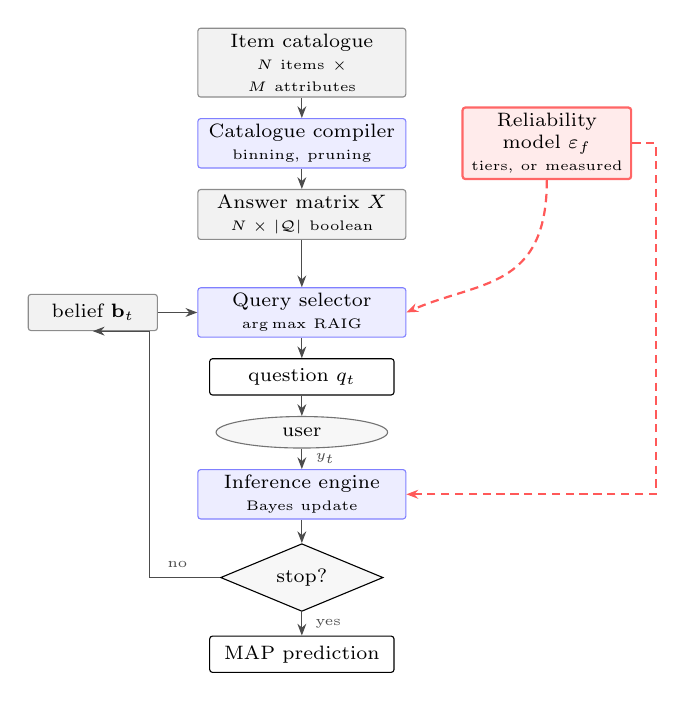
\begin{tikzpicture}[node distance=2.6mm]
\node[fdata, text width=25mm] (cat) {Item catalogue\\{\tiny $N$ items $\times$ $M$ attributes}};
\node[fproc, text width=25mm, below=of cat] (comp)
  {Catalogue compiler\\{\tiny binning, pruning}};
\node[fdata, text width=25mm, below=of comp] (X)
  {Answer matrix $X$\\{\tiny $N\times|\Qset|$ boolean}};
\node[frel, text width=20mm, right=7mm of comp] (rel)
  {Reliability\\model $\varepsilon_f$\\{\tiny tiers, or measured}};
\node[fproc, text width=25mm, below=6mm of X] (sel)
  {Query selector\\{\tiny $\arg\max$ RAIG}};
\node[fdata, text width=15mm, left=5mm of sel] (bel) {belief $\bb_t$};
\node[fbox, text width=22mm, below=of sel] (q) {question $q_t$};
\node[fuser, text width=14mm, below=of q] (user) {user};
\node[fproc, text width=25mm, below=of user] (inf)
  {Inference engine\\{\tiny Bayes update}};
\node[fdec, text width=13mm, below=3mm of inf] (term) {stop?};
\node[fbox, text width=22mm, below=3mm of term] (out) {MAP prediction};

\draw[far] (cat) -- (comp);
\draw[far] (comp) -- (X);
\draw[far] (X) -- (sel);
\draw[far] (bel) -- (sel);
\draw[far] (sel) -- (q);
\draw[far] (q) -- (user);
\draw[far] (user) -- node[right, font=\tiny, xshift=0.5mm] {$y_t$} (inf);
\draw[far] (inf) -- (term);
\draw[far] (term) -- node[right, font=\tiny, xshift=0.5mm] {yes} (out);
\draw[far] (term.west) -- ++(-9mm,0) node[above, font=\tiny, pos=0.6] {no}
           |- (bel.south);
\draw[frar] (rel.south) .. controls +(0,-14mm) and +(9mm,4mm) .. (sel.east);
\draw[frar] (rel.east) -- ++(3mm,0) |- (inf.east);
\end{tikzpicture}
\caption{System architecture. The reliability model is consumed by both the
selector and the inference engine (dashed); existing systems typically consume
it in the latter only, which is the omission this work addresses.}
\label{fig:arch}
\end{figure}
%----------------------------------------------------------------------

\subsection{Algorithms}

Algorithms~\ref{alg:select}--\ref{alg:eval} give the procedure. Selection is
one matrix--vector product and a constant number of vectorised transforms.
Every selector is a pure function of belief, question matrix and reliability
vector, with no internal state; sessions are driven entirely by an externally
supplied random stream. This is not incidental tidiness. It is what allows the
same target and the same noise realisation to be replayed across every method
under comparison, which in turn is what licenses paired statistical testing.

\begin{algorithm}[t]
\caption{Reliability-aware query selection}
\label{alg:select}
\begin{algorithmic}[1]
\Require belief $\bb$, answer matrix $X \in \{0,1\}^{N \times |\Qset|}$,
per-question crossover $\hat{\boldsymbol\varepsilon}$, asked mask $U$
\Ensure index of the next question
\State $\mathbf{p} \gets \bb^{\!\top} X$
  \Comment{split mass of all questions, one product}
\State $\tilde{\mathbf{p}} \gets \mathbf{p} \odot (1-\hat{\boldsymbol\varepsilon})
   + (1-\mathbf{p}) \odot \hat{\boldsymbol\varepsilon}$
\State $\mathbf{s} \gets \Hb(\tilde{\mathbf{p}}) - \Hb(\hat{\boldsymbol\varepsilon})$
\If{modelling abstention}
  \State $\mathbf{s} \gets (1-\hat{\boldsymbol\delta}) \odot \mathbf{s}$
    \Comment{Eq.~\eqref{eq:erasure}}
\EndIf
\State $s_j \gets -\infty$ for all $j$ with $U_j = 1$
\State \Return $\arg\max_j s_j$
\end{algorithmic}
\end{algorithm}

\begin{algorithm}[t]
\caption{Belief update under BSC$(\hat\varepsilon)$}
\label{alg:update}
\begin{algorithmic}[1]
\Require belief $\bb$, answer column $\bx_q$, observation $y$, crossover $\hat\varepsilon$
\If{$y$ is an erasure} \State \Return $\bb$ \Comment{no information} \EndIf
\State $\ell_c \gets 1-\hat\varepsilon$ if $x_q(c)=y$ else $\hat\varepsilon$, for all $c$
\State $\bb' \gets \bb \odot \boldsymbol\ell$; \quad $Z \gets \sum_c b'_c$
\If{$Z = 0$} \Comment{reachable only at $\hat\varepsilon=0$}
  \State \Return $\bb$ \Comment{stated convention; see Prop.~\ref{prop:limit}}
\EndIf
\State \Return $\bb' / Z$
\end{algorithmic}
\end{algorithm}

\begin{algorithm}[t]
\caption{Identification session}
\label{alg:session}
\begin{algorithmic}[1]
\Require catalogue, target $c^\ast$, budget $T$, selector $\pi$,
assumed $\hat{\boldsymbol\varepsilon}$, true $\boldsymbol\varepsilon$,
random stream $u_{1:T}$
\State $\bb \gets$ uniform; $U \gets \mathbf{0}$
\For{$t = 1$ \textbf{to} $T$}
  \State $q \gets \pi(\bb, X, \hat{\boldsymbol\varepsilon}, U)$; $U_q \gets 1$
  \State $y \gets x_q(c^\ast)$
  \If{$u_t < \varepsilon_{f(q)}$} $y \gets 1-y$ \Comment{answer error} \EndIf
  \State $\bb \gets$ \textsc{Update}$(\bb, \bx_q, y, \hat\varepsilon_{f(q)})$
\EndFor
\State \Return $\arg\max_c \bb(c)$
\end{algorithmic}
\end{algorithm}

\begin{algorithm}[t]
\caption{Paired evaluation with common random numbers}
\label{alg:eval}
\begin{algorithmic}[1]
\Require methods $\mathcal{M}$, trials $R$, seeds $S$, budget $T$
\For{each seed $s \in S$}
  \State draw targets $c^\ast_{1:R}$ and streams $u_{1:R,1:T}$ from seed $s$
  \For{$i = 1$ \textbf{to} $R$}
    \For{each $m \in \mathcal{M}$}
      \State record outcome of \textsc{Session}$(c^\ast_i, u_{i,\cdot}, m)$
    \EndFor
  \EndFor
\EndFor
\State \Return per-trial outcomes for paired inference
\end{algorithmic}
\end{algorithm}

One implementation detail is omitted from Algorithm~\ref{alg:select} because it
never fires in our experiments and stating it inline would obscure the
selection rule. A method restricted to a subset of attributes could in
principle exhaust its allowed pool before the budget is spent; the
implementation then falls back to the unrestricted unasked pool rather than
returning nothing. With $T=20$ and at least $126$ allowed questions for every
method including the restricted baseline, this branch is unreachable in every
run reported here, and the restricted baseline's poor showing is therefore not
an artefact of it.

Sharing $u_{i,\cdot}$ across methods in Algorithm~\ref{alg:eval} is deliberate.
Methods diverge in which questions they ask and therefore in which crossover
probabilities they face, but they consult the same underlying draws, so
differences in outcome are attributable to question choice rather than to
sampling luck. This substantially reduces variance relative to independent
sampling and permits exact paired testing~\cite{mcnemar1947}.

\subsection{Complexity}

Let $|\Qset|$ be the number of compiled questions. Selection is one
matrix--vector product and a constant number of vectorised transforms, hence
$O(N|\Qset|)$ time and $O(|\Qset|)$ working memory; the update is $O(N)$. A
session of $T$ turns costs $O(TN|\Qset|)$, and the compiled matrix occupies
$N|\Qset|$ bits. Table~\ref{tab:complexity} summarises. Critically, RAIG and
classical IG have identical asymptotic complexity, and the constant is
negligible too: the correction adds one elementwise affine map and one
subtraction on a vector of length $|\Qset|$ to a matrix--vector product costing
$O(N|\Qset|)$, so the expected relative overhead is $1/N$, here
$1.3\times10^{-5}$. Section~\ref{sec:results-efficiency} reports what happens
when one tries to measure a difference that small on a shared machine.

\begin{table}[t]
\caption{Complexity per operation. RAIG and classical IG differ only in the
score transform, which is $O(|\Qset|)$ for both.}
\label{tab:complexity}
\centering
\footnotesize
\begin{tabular}{@{}lll@{}}
\toprule
\textbf{Operation} & \textbf{Time} & \textbf{Memory} \\
\midrule
Catalogue compilation & $O(NM\bar{V})$ & $O(N|\Qset|)$ bits \\
Split-mass computation & $O(N|\Qset|)$ & $O(|\Qset|)$ \\
Score transform (IG or RAIG) & $O(|\Qset|)$ & $O(|\Qset|)$ \\
Belief update & $O(N)$ & $O(N)$ \\
Full session & $O(TN|\Qset|)$ & $O(N|\Qset|)$ bits \\
\bottomrule
\end{tabular}
\end{table}

\subsection{Implementation and Reproducibility}

The reference implementation is Python~3.13 against NumPy, pandas and SciPy;
no deep-learning framework is required, and the entire selection and inference
path is dense linear algebra. Catalogue compilation materialises one boolean
column per non-degenerate attribute--value pair; questions true of every item
or of none are discarded at compile time, since they carry zero information
under either criterion.

The engineering decision with the largest downstream effect is the separation
of the assumed crossover $\hat{\boldsymbol\varepsilon}$ from the true crossover
$\boldsymbol\varepsilon$ in the session signature. The simulator draws errors
from the latter; the method sees only the former. Conflating them---the natural
shortcut---would make every reported result circular, because the method would
be evaluated against a user whose behaviour it defines. Keeping them distinct
is what makes the misspecification studies of
Sections~\ref{sec:results-ensemble} and~\ref{sec:results-corruption} possible
at all.

\emph{Determinism.} The BLAS thread count is pinned to one before NumPy is
imported. This is a correctness requirement, not a performance tweak. A
multi-threaded matmul sums $(|\Qset|,N)\times(N,\cdot)$ in a shape-dependent
order, so the split-mass vector differs in the last float32 unit in the last
place between runs with different batch shapes; selection is an argmax over
that vector, near-ties are common in a catalogue with many equal-mass
questions, and a single different question at turn one sends the entire session
down a different path. Pinning to one thread makes every run bitwise
reproducible and---verified empirically as a gate test---makes the per-method
results of a run with $M$ methods identical to those of a run with any subset
of them. That property is what allows a new method to be added to an existing
comparison without re-running the incumbents, and it is worth the modest cost
of stating. On our hardware it is also faster, the matmul being memory-bound.

%=============================================================================
\section{Experimental Setup}
\label{sec:setup}
%=============================================================================

Every number reported in this paper comes from the same harness, described in
Section~\ref{sec:system}, run under the protocol fixed here. The protocol is
stated in full before any result is shown because several of the choices---the
budget, the paired sampling, the separation of assumed from true
reliability---determine what the results can and cannot be read to mean.

\subsection{Catalogues}
\label{sec:catalogues}

We use three real catalogues from three domains and one synthetic family.
Table~\ref{tab:catalogues} summarises them.

\emph{Music.} A catalogue of $79{,}803$ tracks described by $21$ attributes,
derived from a public audio-features corpus and used as the item table of a
deployed Akinator-style music identification system. Eleven of the attributes
are discretisations of continuous audio descriptors (danceability, energy,
valence, acousticness, instrumentalness, liveness, speechiness, loudness,
tempo, popularity, duration); the remainder are natively categorical metadata
(genre, language, content rating, artist type, release type, track version) or
music-theoretic labels (key, mode, time signature). This mixture is the
structure the mechanism of Section~\ref{sec:discretisation-theory} requires,
and it is why this catalogue is the primary one.

\emph{Mushroom.} UCI Agaricus-Lepiota~\cite{uci}, $8{,}124$ specimens by $21$ usable
categorical attributes, cast as field identification by a forager. Every
attribute is natively categorical, so the discretisation mechanism cannot
operate. The catalogue is nonetheless a genuine test rather than a formality,
because its two most informative attributes---odour, and colour names drawn
from nine to twelve options---are the two classic unreliable human perceptual
judgements. If high information gain concentrated on hard-to-answer attributes
for reasons other than binning, this is where it would show.

\emph{Dermatology.} UCI Dermatology~\cite{uci,guvenir1998}, $366$ cases by $34$ attributes, cast as
differential narrowing by a triage questioner with the patient as oracle. This
is the one catalogue whose reliability annotation we did not invent: the
dataset documentation itself partitions attributes into clinical and
histopathological, and a histopathological attribute is by construction one the
patient cannot answer at all, since it requires a biopsy and a microscope. Our
annotation refines that documented split by asking who can answer from what
evidence. The single continuous column, age, is banded into quartiles.

\emph{Synthetic.} A family in which the rank correlation between an attribute's
apparent informativeness and its reliability is a control knob, used in
Section~\ref{sec:results-synthetic} to turn the randomised and adversarial
controls---which are two isolated points on that axis---into a continuum.

\begin{table}[t]
\caption{Catalogues. $|\Qset|$ is the number of compiled one-versus-rest
questions after degenerate questions are dropped. The entropy floor is
$\log_2$ of the number of distinct attribute vectors, i.e.\ the information
that must be acquired even with perfect answers; $T_{\min}$ is the
capacity-corrected budget bound~\eqref{eq:budget} under each catalogue's
reliability annotation.}
\label{tab:catalogues}
\centering
\footnotesize
\begin{tabular}{@{}lrrrrr@{}}
\toprule
\textbf{Catalogue} & \textbf{$N$} & \textbf{$M$} & \textbf{$|\Qset|$} &
\textbf{floor} & \textbf{$T_{\min}$} \\
\midrule
Music        & 79{,}803 & 21 & 193 & 16.23 & 20.15 \\
Mushroom     & 8{,}124  & 21 & 116 & 12.99 & 16.12 \\
Dermatology  & 366      & 34 & 134 & 8.52  & 10.58 \\
\bottomrule
\end{tabular}
\end{table}

The music catalogue is not perfectly identifiable, and this bounds every
accuracy we report. Its $79{,}803$ tracks occupy $77{,}069$ distinct attribute
vectors, so $93.7\%$ of items are uniquely identifiable and the largest
equivalence class holds $11$ indistinguishable tracks. No method, with any
budget and a perfect user, can exceed $96.6\%$ top-1 accuracy on it; the clean
condition confirms that the best methods reach exactly that ceiling.

\subsection{Attribute Inventory}
\label{sec:attributes}

Table~\ref{tab:attributes} lists the music attributes with their annotated
tier, their maximum one-versus-rest information gain in the catalogue as
shipped, and the same quantity after the eleven continuous sources are
re-discretised into four equal-population quantile bins. The second column is
the operative one for Section~\ref{sec:results-bias}; the third exists because
it is the clean instantiation of Proposition~\ref{prop:discretisation}, and it
is where every re-binned attribute reports exactly $\Hb(1/4)=0.811$ bits,
regardless of what the attribute means.

Two features of the table should be noted in advance. First, the shipped
catalogue's continuous attributes are \emph{not} equal-population bins: they
were cut at fixed semantic thresholds by the original pipeline, so their split
masses vary and their maximum information gain ranges from $0.231$ to $1.000$
rather than sitting at $\Hb(1/5)$. The bias in the shipped catalogue is
therefore not an artefact of our own preprocessing---we did not do the
binning---and the four-bin column shows what happens when the binning is made
textbook-clean, which is that the bias strengthens
(Section~\ref{sec:results-bias}). Second, genre carries $113$ values and a
maximum one-versus-rest information gain of $0.097$ bits: it is the most
discriminative attribute in the catalogue by any reasonable measure and the
least attractive to a criterion that maximises binary entropy. That single row
is the whole problem in miniature.

\begin{table}[t]
\caption{Music attributes. $|V|$ is the number of distinct values;
$\max\Hb$ is the largest one-versus-rest binary entropy at a uniform belief;
$\max\Hb^{(4)}$ is the same after re-discretising the underlying continuous
column into four equal-population bins (``---'' where the attribute has no
continuous source). Release type is degenerate in this catalogue (a single
value) and compiles to no questions.}
\label{tab:attributes}
\centering
\footnotesize
\begin{tabular}{@{}llrrr@{}}
\toprule
\textbf{Attribute} & \textbf{Tier} & \textbf{$|V|$} &
\textbf{$\max\Hb$} & \textbf{$\max\Hb^{(4)}$} \\
\midrule
genre            & objective & 113 & 0.097 & --- \\
language         & objective & 2   & 0.446 & --- \\
content rating   & objective & 2   & 0.424 & --- \\
artist type      & objective & 4   & 0.834 & --- \\
track version    & objective & 5   & 0.424 & --- \\
release type     & objective & 1   & ---   & --- \\
\midrule
popularity       & semi & 5 & 0.958 & 0.811 \\
duration         & semi & 5 & 0.939 & 0.811 \\
acousticness     & semi & 5 & 0.999 & 0.811 \\
instrumentalness & semi & 5 & 0.819 & 0.811 \\
liveness         & semi & 5 & 0.933 & 0.811 \\
speechiness      & semi & 3 & 0.231 & 0.811 \\
loudness         & semi & 5 & 1.000 & 0.811 \\
\midrule
mood             & subjective & 5 & 1.000 & --- \\
tempo            & subjective & 5 & 0.902 & 0.811 \\
danceability     & subjective & 5 & 0.957 & 0.811 \\
energy           & subjective & 5 & 0.924 & 0.811 \\
valence          & subjective & 5 & 0.804 & 0.811 \\
key              & subjective & 4 & 0.896 & --- \\
mode             & subjective & 2 & 0.947 & --- \\
time signature   & subjective & 3 & 0.496 & --- \\
\bottomrule
\end{tabular}
\end{table}

\subsection{Baselines}
\label{sec:baselines}

A comparison of ``information gain'' against ``a learned policy'' confounds two
independent choices: how the next question is selected, and how the answer is
absorbed. Proposition~\ref{prop:limit} shows the second choice is a limit of one
model rather than a different model, so the two can and should be crossed. Our
nine methods do that, and are listed in Table~\ref{tab:baselines}.

\begin{table}[t]
\caption{Methods. ``Selector'' is the rule that chooses the next question;
``update'' is how the answer is absorbed; $\hat\varepsilon$ is what the method
assumes about answer reliability. Hard elimination is
$\hat\varepsilon \equiv 0$ (Proposition~\ref{prop:limit}), so the selector and
update columns are not independent for that row alone.}
\label{tab:baselines}
\centering
\scriptsize
\begin{tabular}{@{}llll@{}}
\toprule
\textbf{Method} & \textbf{Selector} & \textbf{Update} & \textbf{$\hat\varepsilon$} \\
\midrule
Random+soft         & uniform random & soft & uniform \\
IG+hard             & $\Hb(p_q)$     & hard & $0$ \\
IG+soft-uniform     & $\Hb(p_q)$     & soft & uniform \\
IG+soft-objective   & $\Hb(p_q)$, objective only & soft & uniform \\
Learned-noiseblind  & ridge value regression & soft & uniform \\
Learned-noiseaware  & ridge value regression & soft & uniform \\
RAIG-empirical      & $\RAIG(q)$     & soft & measured \eqref{eq:discordance} \\
RAIG-tiered         & $\RAIG(q)$     & soft & 3-tier annotation \\
RAIG-oracle         & $\RAIG(q)$     & soft & true $\varepsilon$ \\
\bottomrule
\end{tabular}
\end{table}

Two further specifications of $\hat\varepsilon$---RAIG-EM, which learns the
crossover vector from interaction logs, and RAIG-psycho, which computes it from
the catalogue's own cut points---are introduced where they are tested
(Sections~\ref{sec:results-em} and~\ref{sec:results-psycho}) rather than here,
because each is evaluated against this nine-method set rather than alongside it.

Three of the nine deserve comment.

\emph{IG+soft-uniform is the honest incumbent.} It is classical information
gain paired with a correct probabilistic belief update at the catalogue-average
crossover. By Proposition~\ref{prop:uniform} its selector is exactly classical
information gain, so the comparison of RAIG-tiered against IG+soft-uniform
isolates the acquisition function with the update held fixed. This is the
pre-registered primary comparison, and the only one we treat as confirmatory.

\emph{IG+soft-objective is the restricted-attribute baseline}, the practitioner
heuristic of simply not asking unreliable questions. It is the baseline that
most directly threatens the method---if discarding subjective attributes
worked, weighting them would be unnecessary---and we report it in every
condition. Its weakness is structural rather than empirical: the six objective
attributes partition the music catalogue into only $1{,}926$ equivalence
classes, the largest holding $932$ tracks, so the strategy has a top-1 accuracy
ceiling of $0.65\%$ however many questions it is given. We state this ceiling
in advance so that its poor showing is not mistaken for a tuning failure.

\emph{The learned policies} are myopic value-regression selectors in the
EAR/CPR mould~\cite{lei2020ear,lei2020cpr}: roll out a behaviour policy, log
state--question features against the realised one-turn reduction in belief
entropy, fit a ridge regressor, and select by the learned score. Training uses
$600$ simulated sessions of $T=20$ turns, giving $12{,}000$ samples over $51$
features, with ridge penalty $\lambda=1$. The two variants differ in exactly
one respect: the noise used to generate the training rollouts. Noiseblind
trains on noiseless rollouts, which is the modelling choice we attribute to
prior work; noiseaware trains under the true heterogeneous noise and can in
principle discover the reliability weighting from data. The feature set
deliberately includes the interaction between split balance and attribute
identity ($\Hb(p) \times$ attribute one-hot), so a linear model over these
features \emph{can} represent a per-attribute discount on balanced splits,
which is precisely what RAIG encodes. Omitting that interaction would have
guaranteed the baseline could not compete and made any win an artefact of
feature design.

\subsection{Noise Conditions}
\label{sec:conditions}

The simulator draws answer errors from a true per-question crossover vector
$\boldsymbol\varepsilon$; every method sees only its own assumed
$\hat{\boldsymbol\varepsilon}$. The two are separate arguments in the session
signature, and conflating them would make every result circular. Seven
conditions are used throughout.

\begin{enumerate}
\item \emph{Clean}: $\varepsilon \equiv 0$. A sanity condition, not a realistic
one. Its purpose is to verify that every method attains the identifiability
ceiling when the model's noise assumption is the only thing that is wrong.
\item \emph{Homogeneous}: $\varepsilon \equiv 0.098$, the catalogue average of
the tier annotation. Answer noise, but no heterogeneity, hence nothing for a
reliability-aware selector to exploit (Proposition~\ref{prop:uniform}).
\item \emph{Heterogeneous} at $\lambda \in \{0.5, 1.0, 1.5\}$:
$\varepsilon_f = \lambda \cdot \varepsilon_{\mathrm{tier}(f)}$, with
$\lambda=1.0$ the primary condition. $\lambda$ scales user noise without
changing its structure, and locating the value at which reliability awareness
begins to pay is the practitioner-facing question of
Section~\ref{sec:results-lambda}.
\item \emph{Randomised}: the attribute-to-$\varepsilon$ assignment is permuted.
The tier annotation is then uninformative about the truth, and the system is
running on an annotation that has been scrambled behind its back.
\item \emph{Adversarial}: $\varepsilon$ is assigned in inverse rank order of
maximum information gain, so the best-splitting attribute becomes the most
reliable. The annotation is now not merely uninformative but wrong in the
direction most damaging to RAIG.
\end{enumerate}

The last two are the conditions under which the theory predicts our method
should lose, and we report them with the same prominence as the conditions in
which it wins. A method that could not be made to fail by inverting its
assumption would be a method whose assumption did no work.

\subsection{Metrics}
\label{sec:metrics}

Top-1 accuracy at the budget is the headline metric because it is what an
identification system is for. It is also the metric most compressed against the
entropy floor at $T=20$, so we report alongside it: top-5 and top-10 accuracy;
the median rank of the true item; mean reciprocal rank; the negative log
posterior of the true item in bits, which is sensitive to belief quality even
when no prediction is correct; and, for the behavioural claim, the mean true
$\varepsilon$ of the questions each method actually chose to ask, together with
the tier composition of those questions. That last pair is the most direct
evidence for or against the bias, because it measures what the selector did
rather than how well it happened to do.

Ranks use the mid-rank convention, $1 + |\{i : b_i > b^\ast\}| +
(|\{i : b_i = b^\ast\}| - 1)/2$. This matters more than it sounds: early in a
session the belief vector carries very large ties, and the optimistic
convention would credit a method for a tie it has not broken.

\subsection{Statistical Protocol}
\label{sec:stats}

Trials are paired by construction. For each trial index the harness draws one
target item and one stream of uniform variates, and every method under
comparison plays that same target against that same stream
(Algorithm~\ref{alg:eval}). Methods diverge in which questions they ask and
therefore in which crossover probabilities they face, but they consult the same
underlying draws, so a difference in outcome is attributable to question choice
rather than to sampling luck. The primary comparison uses $R=300$ trials at
each of three seeds, $n=900$ paired trials per cell.

Significance is assessed with the exact (binomial) McNemar
test~\cite{mcnemar1947} on the discordant pairs, which is the appropriate test
for paired binary outcomes and does not rely on a normal approximation that
would be poor at these discordance counts. Within each condition the family of
comparisons against the reference method is corrected by the Holm step-down
procedure~\cite{holm1979}. Confidence intervals on accuracies and on paired
differences are bootstrap percentile intervals over $10{,}000$ resamples.

One comparison is designated primary in advance: RAIG-tiered against
IG+soft-uniform, top-1 accuracy, heterogeneous $\lambda=1.0$, $T=20$. Every
other comparison in this paper is exploratory, and we label the tables
accordingly rather than reporting a wall of asterisks and letting the reader
assume they were all planned.

%=============================================================================
\section{Results}
\label{sec:results}
%=============================================================================

\subsection{The Bias Is Present and Is Made by the Discretiser}
\label{sec:results-bias}

The first claim is diagnostic and does not involve running a single session:
in the music catalogue, apparent informativeness and annotated answerability
are negatively related.

The natural way to report it is a Spearman correlation between per-attribute
maximum information gain and annotated reliability, which over the twenty
non-degenerate attributes gives $\rho = -0.438$ ($p = 0.054$). That statistic
is the wrong instrument for the data. Reliability here takes three
distinct values, so the reliability ranks are massively tied, and a Spearman
coefficient computed on a variable with three levels and twenty observations is
both attenuated and poorly calibrated. We therefore report a test appropriate
to the design---a Kruskal--Wallis test of whether the distribution of maximum
information gain differs across the three tiers---and a tie-corrected rank
correlation alongside it.

The Kruskal--Wallis test rejects: $H = 7.23$, $p = 0.027$. Kendall's $\tau_b$,
which is tie-corrected, gives $-0.311$ ($p = 0.088$). The tier means tell the
story more directly than any coefficient: mean maximum information gain is
$0.445$ bits for objective attributes against $0.840$ for semi-objective and
$0.866$ for subjective. Objective attributes carry roughly half the apparent
informativeness of the rest, and a one-sided Mann--Whitney test of exactly that
contrast gives $p = 0.0027$. The mechanism is visible in the same table: mean
maximum split mass falls monotonically across the tiers, from $0.696$ for
objective attributes through $0.587$ for semi-objective ones to $0.451$ for
subjective ones---and $0.5$ is the value that maximises $\Hb$. Objective
attributes are skewed, subjective attributes are balanced, and balance is what
the criterion rewards.

\emph{The discretiser is responsible.} Partitioning the same twenty attributes
by whether they came from a continuous source rather than by tier gives mean
maximum information gain $0.861$ for binned attributes against $0.618$ for
natively categorical ones (Mann--Whitney $p = 0.047$), while the mean annotated
crossover of the binned group is $0.205$ against $0.150$ for the categorical
group. The binned attributes are simultaneously the most attractive to the
criterion and the least reliable, which is precisely
Proposition~\ref{prop:discretisation} acting on perceptual quantities.

\emph{Refining the binning strengthens the bias, as predicted.} Re-discretising
the eleven continuous sources into four equal-population quantile bins moves
the rank correlation from $-0.438$ ($p = 0.054$) to $-0.613$ ($p = 0.0041$).
Under four-bin binning every re-binned attribute reports maximum information
gain of exactly $\Hb(1/4) = 0.811$ bits---the equality
Proposition~\ref{prop:discretisation} asserts, visible in the last column of
Table~\ref{tab:attributes}---so the ordering among attributes becomes almost
entirely a question of which ones passed through the discretiser. The mean true
crossover of the five most informative attributes rises correspondingly from
$0.210$ to $0.246$, against a catalogue average of $0.180$. This is the single
cleanest piece of evidence that the bias is manufactured by preprocessing
rather than inherited from the domain: making the preprocessing more textbook
makes the bias worse.

\subsection{Primary Comparison}
\label{sec:results-main}

The pre-registered comparison is RAIG-tiered against IG+soft-uniform, top-1
accuracy, heterogeneous $\lambda = 1.0$, at a budget of $T = 40$ questions and
$n = 900$ paired trials. Table~\ref{tab:primary} reports it for all nine
methods.

\emph{On the choice of budget.} Corollary~\ref{cor:budget} puts the minimum
sufficient budget for this catalogue at $20.15$ questions. A system run at
$T=20$ is therefore operating exactly on the information-theoretic boundary,
where even a method with perfect knowledge of $\boldsymbol\varepsilon$ can
barely succeed, and where every method is compressed against the floor. That is
a stress test, and we report it as one throughout
Section~\ref{sec:robustness}; it is not a sensible headline. Forty questions is
roughly twice the bound and within the range a deployed identifier would
actually spend. The choice cannot be read as selecting a flattering operating
point, because Section~\ref{sec:results-budget} shows the advantage
\emph{widens} monotonically with budget: $T=20$ was the conservative reading of
our own result, not the favourable one.

\begin{table}[t]
\caption{Primary comparison at $T=40$, heterogeneous $\lambda = 1.0$,
$n = 900$ paired trials. $\bar\varepsilon_{\text{asked}}$ is the mean true
crossover of the questions the selector chose, against a catalogue average of
$0.098$; ``subj.'' is the share of its budget spent on the subjective tier.
RAIG-tiered and RAIG-oracle coincide exactly here because the tier annotation
\emph{is} the truth in this condition by construction; they separate in the
conditions of Table~\ref{tab:main}, where it is not.}
\label{tab:primary}
\centering
\footnotesize
\begin{tabular}{@{}lrrrrr@{}}
\toprule
\textbf{Method} & \textbf{top-1} & \textbf{95\% CI} & \textbf{top-5} &
\textbf{$\bar\varepsilon_{\text{asked}}$} & \textbf{subj.} \\
\midrule
Random+soft        & 0.22  & $[0.00, 0.56]$   & 1.56  & 0.099 & 17.8 \\
IG+hard            & 2.11  & $[1.22, 3.11]$   & 2.22  & 0.102 & 19.0 \\
IG+soft-uniform    & 16.56 & $[14.11, 19.00]$ & 27.22 & 0.197 & 46.1 \\
IG+soft-objective  & 0.33  & $[0.00, 0.78]$   & 1.89  & 0.030 & 0.0  \\
Learned-noiseblind & 18.89 & $[16.33, 21.44]$ & 30.11 & 0.182 & 42.3 \\
Learned-noiseaware & 13.89 & $[11.67, 16.22]$ & 23.33 & 0.211 & 50.2 \\
RAIG-empirical     & 10.22 & $[8.33, 12.22]$  & 20.56 & 0.214 & 53.6 \\
\textbf{RAIG-tiered} & \textbf{26.56} & $[23.78, 29.44]$ & \textbf{44.78} & 0.134 & 21.2 \\
RAIG-oracle        & 26.56 & $[23.78, 29.44]$ & 44.78 & 0.134 & 21.2 \\
\bottomrule
\end{tabular}
\end{table}

\emph{The primary result.} RAIG-tiered reaches $26.56\%$ top-1 accuracy
($95\%$ CI $[23.78, 29.44]$) against IG+soft-uniform's $16.56\%$
($[14.11, 19.00]$). The paired difference is $+10.00\pp$
($[+6.89, +13.11]$) on $214$ discordant pairs, exact McNemar
$p = 6.6\times10^{-10}$, Holm-adjusted $p = 2.0\times10^{-9}$. All eight
comparators are beaten at Holm-adjusted $\alpha = 0.05$
(Table~\ref{tab:mcnemar}). Top-5 accuracy is $44.78\%$ against $27.22\%$, and
the median rank of the true item is $8.8$ against $59.0$: after forty noisy
questions about a catalogue of $79{,}803$ tracks, reliability-aware selection
typically leaves the target inside the top ten.

\emph{The learned policy is the strongest baseline at this budget, and still
loses.} Learned-noiseblind reaches $18.89\%$, ahead of classical information
gain, which it was not at $T=20$; the extra budget gives a policy with
attribute-level features room to exploit them. It remains $7.67\pp$ behind
RAIG-tiered ($p = 2.1\times10^{-5}$ after correction), and its noise-aware
sibling is worse still, for the reason Section~\ref{sec:results-learned} gives.

Table~\ref{tab:main} reports top-1 accuracy for all nine methods across all
seven noise conditions. That sweep is run at $T=20$, the floor budget: it exists
to show where the method wins and where it fails, and the failures are clearest
at the harder operating point. Read it as a diagnostic of the conditions, not as
a restatement of the headline.

\begin{table*}[t]
\caption{Condition sweep: top-1 accuracy (\%) at the floor budget $T=20$,
$n=900$ paired trials per cell. Het.\ $\lambda$ scales the tiered crossover
values. This table is a diagnostic of \emph{where} reliability weighting helps
and where it hurts, deliberately reported at the harder budget; the headline
comparison is Table~\ref{tab:primary}. \textbf{Bold} marks the condition
corresponding to the primary comparison. RAIG-tiered and RAIG-oracle coincide
exactly in the heterogeneous columns because the tier annotation \emph{is} the
truth there by construction; they separate in the clean, homogeneous,
randomised and adversarial columns, where it is not.}
\label{tab:main}
\centering
\footnotesize
\begin{tabular}{@{}lrrrrrrr@{}}
\toprule
\textbf{Method} & \textbf{Clean} & \textbf{Homog.} &
\textbf{Het.\ 0.5} & \textbf{Het.\ 1.0} & \textbf{Het.\ 1.5} &
\textbf{Rand.} & \textbf{Adv.} \\
\midrule
Random+soft        & 0.89  & 0.22  & 0.56  & 0.22          & 0.11 & 0.00  & 0.00  \\
IG+hard            & 96.56 & 20.33 & 17.78 & 2.00          & 0.11 & 4.22  & 11.33 \\
IG+soft-uniform    & 96.33 & 28.00 & 22.89 & \textbf{3.22} & 0.11 & 8.78  & 16.89 \\
IG+soft-objective  & 0.56  & 0.22  & 0.56  & 0.33          & 0.33 & 0.00  & 0.00  \\
Learned-noiseblind & 92.89 & 23.89 & 22.22 & 4.00          & 0.11 & 7.00  & 12.00 \\
Learned-noiseaware & 90.11 & 23.00 & 19.11 & 3.11          & 0.22 & 6.89  & 10.89 \\
RAIG-empirical     & 52.33 & 12.89 & 11.56 & 2.00          & 0.11 & 4.11  & 3.11  \\
RAIG-tiered        & 41.89 & 10.67 & 17.56 & \textbf{8.33} & 3.00 & 5.33  & 3.44  \\
RAIG-oracle        & 96.56 & 28.00 & 30.33 & 8.33          & 3.00 & 18.11 & 24.67 \\
\bottomrule
\end{tabular}
\end{table*}

\emph{At the floor budget the same ordering holds, compressed.} In the
$\lambda = 1.0$ column of Table~\ref{tab:main}, RAIG-tiered reaches $8.33\%$
($95\%$ CI $[6.56, 10.22]$) against IG+soft-uniform's $3.22\%$
($[2.11, 4.44]$), a paired difference of $+5.11\pp$ ($[+3.11, +7.22]$) on $94$
discordant pairs, exact McNemar $p = 2.2\times10^{-6}$. Every comparator is
beaten after Holm correction here too (Table~\ref{tab:mcnemar}). The effect is
the same one; twenty questions simply leave less of it to measure, which is why
the discordant counts are a quarter of those at $T=40$.

\begin{table}[t]
\caption{Paired comparisons against RAIG-tiered at heterogeneous
$\lambda = 1.0$, $n = 900$, at the headline budget $T=40$ and at the floor
budget $T=20$. $\Delta$ is RAIG-tiered minus the comparator with a bootstrap
$95\%$ interval, ``disc.'' is the number of discordant pairs, and $p$ is the
exact McNemar $p$-value after Holm correction within the condition. Only the
IG+soft-uniform row is confirmatory; the rest are exploratory.}
\label{tab:mcnemar}
\centering
\tiny
\begin{tabular}{@{}lrrrrrr@{}}
\toprule
& \multicolumn{3}{c}{$T=40$} & \multicolumn{3}{c}{$T=20$} \\
\cmidrule(lr){2-4}\cmidrule(lr){5-7}
\textbf{Comparator} & \textbf{$\Delta$} & \textbf{disc.} &
\textbf{$p_{\text{Holm}}$} & \textbf{$\Delta$} & \textbf{disc.} &
\textbf{$p_{\text{Holm}}$} \\
\midrule
Random+soft        & $+26.33$ & 239 & $4.4\times10^{-69}$ & $+8.11$ & 77 & $3.2\times10^{-19}$ \\
IG+soft-objective  & $+26.22$ & 242 & $4.7\times10^{-66}$ & $+8.00$ & 76 & $5.4\times10^{-19}$ \\
IG+hard            & $+24.44$ & 238 & $1.6\times10^{-55}$ & $+6.33$ & 85 & $1.2\times10^{-9}$  \\
RAIG-empirical     & $+16.33$ & 217 & $1.9\times10^{-24}$ & $+6.33$ & 71 & $7.6\times10^{-12}$ \\
Learned-noiseaware & $+12.67$ & 212 & $6.7\times10^{-15}$ & $+5.22$ & 83 & $8.4\times10^{-7}$  \\
IG+soft-uniform    & $+10.00$ & 214 & $2.0\times10^{-9}$  & $+5.11$ & 94 & $6.6\times10^{-6}$  \\
Learned-noiseblind & $+7.67$  & 241 & $2.1\times10^{-5}$  & $+4.33$ & 89 & $8.6\times10^{-5}$  \\
RAIG-oracle        & $0.00$   & 0   & $1.00$              & $0.00$  & 0  & $1.00$ \\
\bottomrule
\end{tabular}
\end{table}

\emph{Where the method loses, and why that is the point.} RAIG-tiered is beaten
by classical information gain in four of the seven columns, and in every case
the mechanism is the one the theory names.

In the \emph{clean} column it collapses to $41.89\%$ against $96.33\%$. The
cause is not a modelling failure but the capacity ceiling of
Corollary~\ref{cor:budget} acting through ties. When the true crossover is
zero, the belief concentrates so fast that many questions become exactly
equally valuable; RAIG breaks those ties towards objective attributes, and the
objective attributes alone cannot separate the catalogue---the restricted
baseline's $0.65\%$ ceiling of Section~\ref{sec:baselines} is the same fact
seen from the other side. Given more budget the deficit closes: at $T=40$
RAIG-tiered reaches $89.3\%$ and at $T=60$, $95.1\%$. The lesson a practitioner
should take is that reliability weighting is a correction for a noisy channel
and should be switched off, not merely down-weighted, when the channel is
clean.

In the \emph{homogeneous} column it also trails ($10.67\%$ against $28.00\%$).
This is the same tie-breaking effect: the truth is uniform, so by
Proposition~\ref{prop:uniform} there is nothing to gain, and the tiered
assumption is simply wrong about a world where every attribute is equally
reliable.

In the \emph{randomised} and \emph{adversarial} columns it loses to
IG+soft-uniform by $3.45\pp$ and $13.45\pp$. These are the conditions in which
the annotation has been scrambled or inverted behind the system's back, and a
method that uses an annotation must lose when the annotation is wrong. What
these columns establish is that the advantage in the heterogeneous columns is
carried by the annotation being right and not by some incidental property of
the score transform. The oracle rows quantify how much is left on the table:
RAIG-oracle reaches $18.11\%$ and $24.67\%$ in those same columns, so the
information is there to be exploited---what is missing is a correct
$\hat\varepsilon$, which is exactly the quantity
Sections~\ref{sec:results-ensemble} and~\ref{sec:results-corruption} probe.

\emph{The annotation-free specification does not work, and the failure is
diagnosable.} RAIG-empirical, which infers $\hat\varepsilon$ from the rate at
which repeated items in the catalogue disagree with each other, reaches
$2.00\%$---worse than the incumbent it was meant to improve on, and beaten by
the tiered specification by $6.33\pp$
($p = 7.6\times10^{-12}$). Table~\ref{tab:asked} says why: it asks questions at
mean crossover $0.204$ and fills $52.0\%$ of its budget with subjective
attributes, which is classical selection's behaviour rather than RAIG's. The
estimator it rests on is dominated by two attributes whose catalogue
instability has nothing to do with answerability---popularity, which genuinely
differs between a single and an album cut, and genre, which is assigned per
playlist rather than per track---and those two are ranked as the least reliable
attributes in the catalogue when a listener answers both of them easily. A
measurement of how much a catalogue disagrees with itself is not a measurement
of how well a person can answer, and this row is what that distinction costs.
Section~\ref{sec:results-em} supplies the annotation-free specification that
does work, by measuring people instead.

\emph{Two internal consistency checks pass.} First, RAIG with a uniform
$\hat\varepsilon$ reproduces IG+soft-uniform trial for trial, as
Proposition~\ref{prop:uniform} requires. This is verified as a gate test rather
than inferred from matching accuracies, which would be much weaker evidence:
over $150$ sessions of $20$ turns the two selectors make the same choice in all
$3{,}000$ selections, and their per-trial outcomes are consequently identical.
It is also the $K=1$ row of the ablation in
Section~\ref{sec:results-ablation}. Second, RAIG-tiered and RAIG-oracle are
\emph{identical}, not merely close, in the three heterogeneous columns ($0$
discordant pairs out of $900$), because at $\varepsilon_f = \lambda\,
\varepsilon_{\mathrm{tier}(f)}$ the tier annotation is the truth up to a scale
that does not change the ranking. They separate wherever it is not, which is
the other four columns.

\subsection{What the Selectors Actually Ask}
\label{sec:results-behaviour}

Accuracy is downstream evidence. The direct evidence for the bias is what each
selector chose to ask, which the harness logs, and it is unambiguous
(Table~\ref{tab:asked}).

\begin{table}[t]
\caption{Behaviour of each selector at heterogeneous $\lambda = 1.0$, $T=40$,
over all $900 \times 40$ selected questions.
$\bar\varepsilon_{\text{asked}}$ is the mean \emph{true} crossover of the
questions chosen; the catalogue average over all compiled questions is
$0.098$. $\overline{\Hb}$ is their mean apparent informativeness. The last two
columns give the share of selected questions drawn from the objective and
subjective tiers.}
\label{tab:asked}
\centering
\footnotesize
\begin{tabular}{@{}lrrrr@{}}
\toprule
\textbf{Method} & \textbf{$\bar\varepsilon_{\text{asked}}$} &
\textbf{$\overline{\Hb}$} & \textbf{obj.\ \%} & \textbf{subj.\ \%} \\
\midrule
Random+soft        & 0.099 & 0.276 & 65.1  & 17.8 \\
IG+hard            & 0.102 & 0.362 & 63.7  & 19.0 \\
IG+soft-uniform    & 0.197 & 0.684 & 18.4  & 46.1 \\
IG+soft-objective  & 0.030 & 0.156 & 100.0 & 0.0  \\
Learned-noiseblind & 0.182 & 0.615 & 26.2  & 42.3 \\
Learned-noiseaware & 0.211 & 0.715 & 11.8  & 50.2 \\
RAIG-empirical     & 0.214 & 0.701 & 13.6  & 53.6 \\
RAIG-tiered        & 0.134 & 0.542 & 40.0  & 21.2 \\
\bottomrule
\end{tabular}
\end{table}

Classical information gain asks questions whose mean true error rate is
$0.197$, against a catalogue average of $0.098$. It does not merely fail to
avoid the unreliable questions: it seeks them out, at twice the rate a
uniformly random selector encounters them, and fills $46.1\%$ of its budget
with subjective attributes while drawing only $18.4\%$ from the objective tier.
Random selection, which optimises nothing, faces a mean crossover of $0.099$
---the catalogue average, as it must. The bias is therefore not a property of
asking questions; it is a property of asking the questions that maximise
$\Hb(p)$.

RAIG-tiered inverts the mix, to $40.0\%$ objective against $21.2\%$ subjective
at a mean crossover of $0.134$, and it pays $0.142$ bits of apparent
informativeness per question for it ($0.542$ against $0.684$). That trade---less
nominal information per question, more actual information per question---is the
entire method, and this table is where it is visible as behaviour rather than
as outcome.

One feature of the table is specific to the longer budget and worth noting,
because it shows the correction is not a blanket ban. At $T=20$ RAIG-tiered
spends only $2.9\%$ of its questions on subjective attributes; at $T=40$ it
spends $21.2\%$. Having exhausted the reliable questions that separate the
catalogue, it returns to the vague ones rather than idling---which is the
behaviour Section~\ref{sec:baselines} argues the restricted-attribute
heuristic gets wrong. An attribute answered correctly seventy per cent of the
time still carries information, and a weighting, unlike an exclusion, can spend
it once the cheap information is gone.

\subsection{Learned Policies Inherit the Blind Spot}
\label{sec:results-learned}

The claim that a learned selection policy trained without a noise model
inherits the bias is, in this paper, not a citation but a measurement.

Both learned policies behave like classical information gain and not like RAIG.
Learned-noiseblind asks questions at mean crossover $0.205$ with $47.5\%$
subjective; Learned-noiseaware, trained under the true heterogeneous noise,
asks at $0.219$ with $53.6\%$ subjective---\emph{worse} than its noiseblind
sibling on both counts. Their accuracies follow: $4.00\%$ and $3.11\%$ against
RAIG-tiered's $8.33\%$, both differences significant after correction.

The reason is visible in the fitted coefficients. The feature set contains the
interaction between split balance and attribute identity, which is the term
through which a linear policy can express ``discount balanced splits on this
attribute''---exactly the RAIG weighting. Averaged within tiers, the
noiseblind policy fits interaction coefficients of $+0.391$ (objective),
$-0.075$ (semi) and $-0.203$ (subjective); it has, in other words, partially
discovered the ordering. The noiseaware policy fits $+0.248$, $-0.074$ and
$-0.062$: a \emph{weaker} preference, in the same direction.

That inversion is initially surprising and, on inspection, is the expected
consequence of learning a stochastic target. The regression target is the
realised one-turn reduction in belief entropy. Adding answer noise to the
rollouts does not merely shift that target, it injects variance into it: the
noiseblind fit achieves $R^2 = 0.41$, the noiseaware fit $R^2 = 0.25$ on the
same $12{,}000$ samples. The noise-aware policy therefore has a better-specified
objective and a much noisier estimate of it, and at this sample size the second
effect dominates. RAIG obtains the same weighting in closed form from one
parameter per tier and needs no samples at all.

We state the scope of this finding carefully. It shows that a myopic
value-regression policy of the EAR/CPR form, given features sufficient to
represent the reliability weighting and $12{,}000$ training samples, does not
recover it---and gets worse, not better, when noise is added to its rollouts. It
does not show that no learned policy could. A policy with a far larger
interaction budget, or one given $\varepsilon$ as an input feature, plainly
could; but a policy given $\varepsilon$ as a feature is a reliability-aware
policy, which is the paper's point rather than a counterexample to it.

\subsection{Budget}
\label{sec:results-budget}

Section~\ref{sec:intro} promised that the choice of $T=20$ would not be allowed
to do the work. Fig.~\ref{fig:budget} and Table~\ref{tab:budget} sweep the
budget from $5$ to $60$
questions in the primary condition. It is an independent run rather than a
re-reading of Table~\ref{tab:main}: a single $T=60$ pass per condition, with
every budget snapshotted along the way so that all curves share one set of
targets and one noise stream, at $n = 450$ paired trials. Its $T=20$ column
therefore need not reproduce Table~\ref{tab:main} exactly, and does not; the
two agree within sampling error, and we report both rather than quietly
harmonising them.

%---------------------------------------------------------------- Fig. budget
\begin{figure}[t]
\centering
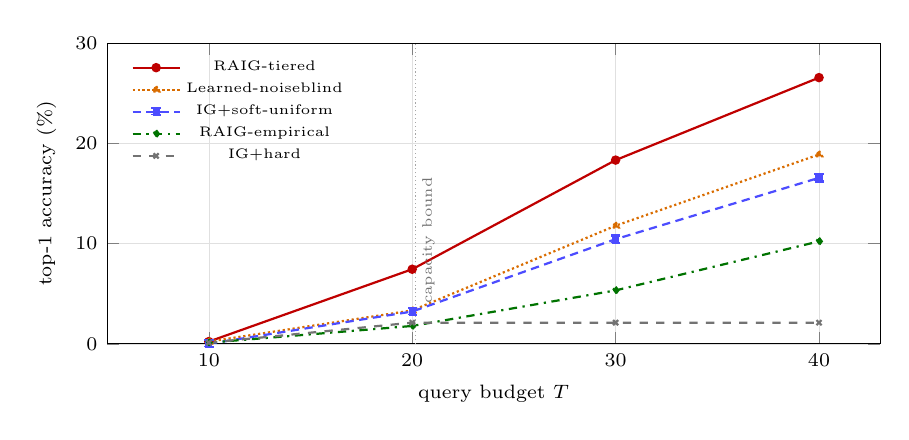
\begin{tikzpicture}
\begin{axis}[
  width=0.94\columnwidth, height=5.4cm,
  xlabel={query budget $T$}, ylabel={top-1 accuracy (\%)},
  xmin=5, xmax=43, ymin=0, ymax=30,
  xtick={10,20,30,40},
  tick label style={font=\scriptsize}, label style={font=\scriptsize},
  legend style={font=\tiny, at={(0.02,0.98)}, anchor=north west, draw=none,
                fill=none, row sep=-1pt},
  grid=major, grid style={black!12, very thin},
  mark size=1.3pt,
]
\addplot[red!75!black, thick, mark=*] coordinates
  {(10,0.22) (20,7.44) (30,18.33) (40,26.56)};
\addlegendentry{RAIG-tiered}
\addplot[orange!85!black, thick, densely dotted, mark=triangle*] coordinates
  {(10,0.22) (20,3.33) (30,11.78) (40,18.89)};
\addlegendentry{Learned-noiseblind}
\addplot[blue!70, thick, densely dashed, mark=square*] coordinates
  {(10,0.00) (20,3.22) (30,10.44) (40,16.56)};
\addlegendentry{IG+soft-uniform}
\addplot[green!45!black, thick, dashdotted, mark=diamond*] coordinates
  {(10,0.11) (20,1.78) (30,5.33) (40,10.22)};
\addlegendentry{RAIG-empirical}
\addplot[black!55, thick, dashed, mark=x] coordinates
  {(10,0.11) (20,2.11) (30,2.11) (40,2.11)};
\addlegendentry{IG+hard}
\draw[black!35, thin, densely dotted] (axis cs:20.15,0) -- (axis cs:20.15,30);
\node[font=\tiny, anchor=west, black!55, rotate=90] at (axis cs:20.8,3)
  {capacity bound};
\end{axis}
\end{tikzpicture}
\caption{Accuracy against query budget at heterogeneous $\lambda=1.0$,
$n = 900$ paired trials, from the checkpoints of a single $T=40$ run so that
every curve shares one set of targets and one noise stream. The advantage of
reliability-aware selection \emph{widens} with budget---$+4.22\pp$ at $T=20$,
$+7.89\pp$ at $T=30$, $+10.00\pp$ at $T=40$---so the floor budget understates
it. The dotted line marks the capacity-corrected bound of
Corollary~\ref{cor:budget}. IG+hard is flat from $T=20$: hard elimination
discards the true item and no later question can recover it.}
\label{fig:budget}
\end{figure}
%----------------------------------------------------------------------

\begin{table}[t]
\caption{Top-1 accuracy (\%) against query budget, heterogeneous
$\lambda = 1.0$, $n = 900$; the data behind Fig.~\ref{fig:budget}. The last two
columns extend the curve to $T=60$ from an independent run at $n=450$, and are
marked separately because they are not from the same sample.}
\label{tab:budget}
\centering
\scriptsize
\begin{tabular}{@{}lrrrrcrr@{}}
\toprule
& \multicolumn{4}{c}{$n=900$} & & \multicolumn{2}{c}{$n=450$} \\
\cmidrule(lr){2-5}\cmidrule(lr){7-8}
\textbf{Method} & \textbf{10} & \textbf{20} & \textbf{30} & \textbf{40} & &
\textbf{50} & \textbf{60} \\
\midrule
Random+soft        & 0.11 & 0.11 & 0.11  & 0.22  & & ---  & ---  \\
IG+hard            & 0.11 & 2.11 & 2.11  & 2.11  & & 2.0  & 2.0  \\
IG+soft-uniform    & 0.00 & 3.22 & 10.44 & 16.56 & & 20.4 & 23.8 \\
IG+soft-objective  & 0.11 & 0.33 & 0.33  & 0.33  & & ---  & ---  \\
Learned-noiseblind & 0.22 & 3.33 & 11.78 & 18.89 & & ---  & ---  \\
Learned-noiseaware & 0.00 & 2.44 & 7.22  & 13.89 & & 20.9 & 24.2 \\
RAIG-empirical     & 0.11 & 1.78 & 5.33  & 10.22 & & 15.1 & 16.0 \\
RAIG-tiered        & 0.22 & 7.44 & 18.33 & 26.56 & & 33.6 & 35.1 \\
\bottomrule
\end{tabular}
\end{table}

Three things follow. First, the advantage is not an artefact of the operating
point: it \emph{widens} with budget, from $+4.22\pp$ at $T=20$ through
$+7.89\pp$ at $T=30$ to $+10.00\pp$ at $T=40$. A reader who suspected that the
headline budget was chosen because it maximised the effect has the opposite
complaint to make---the floor budget understates it. Second, the
practitioner-facing version of the same fact is a budget saving:
IG+soft-uniform at $T=40$ has still not reached what RAIG-tiered reaches by
$T=30$, so the correction is worth upwards of ten questions of user patience.
Third, hard elimination is not merely worse but \emph{terminally} worse: its
accuracy is flat from $T=20$, because a single contradicted answer removes the
true item permanently. The belief-quality metrics say the same thing more
starkly---at $T=40$ IG+hard records a negative log posterior of $97.45$ bits on
the true item, having assigned the correct answer essentially zero probability,
against $9.87$ for IG+soft-uniform and $6.41$ for RAIG-tiered.

Because top-1 accuracy is the most compressed metric at low budgets, we also
report rank-based ones, where the ordering is unchanged and the margins are
larger. At $T=40$ RAIG-tiered attains a median rank of $8.8$ for the true item
against $59.0$ for IG+soft-uniform, a mean reciprocal rank of $0.347$ against
$0.216$, and top-10 accuracy of $51.9\%$ against $31.4\%$. On a catalogue of
$79{,}803$ items, a median rank under ten after forty noisy questions is the
substantive result.

\subsection{Accuracy as a Function of Catalogue Size}
\label{sec:results-size}

Catalogue size is a parameter of the task, not of the method, and the primary
comparison fixes it at the largest value we have. Eighty thousand tracks at a
budget near the capacity bound is the hardest configuration this task admits,
and it is the reason the headline accuracies are what they are. Many deployed
interactive identifiers are not in that regime: a product finder's catalogue, a
fault taxonomy or a game's character set is more often thousands of items than
tens of thousands. This subsection reports what the same methods, with the same
annotation, do across that range.

\emph{What this experiment is not.} It is not cross-validation and must not be
read as such. Nothing here is fitted, so there is no train/test split to make:
the catalogue \emph{is} the hypothesis space, and drawing a subset of it does
not estimate generalisation, it shrinks the search problem. The entropy floor
falls as $\log_2 N$, so accuracy rises for a purely mechanical reason, and a
subset accuracy is not an estimate of the full-catalogue accuracy. What the
sweep does establish is how the difficulty scales, and---the point that
matters---whether the advantage this paper reports survives at every scale.

\emph{Design.} For each seed we draw an independent uniform subset without
replacement and compile it from scratch, so split masses, degenerate questions
and identifiability are all recomputed; the target is drawn from that subset.
Averaging over seeds therefore averages over the draw as well as over targets.
Because a smaller catalogue has fewer colliding attribute vectors, the
attainable ceiling also rises, and Table~\ref{tab:size} reports it per size so
that an easier search is not confused with a higher ceiling.

\begin{table}[t]
\caption{Top-1 accuracy (\%) across catalogue size and query budget,
heterogeneous $\lambda = 1.0$, $n = 600$ paired trials per cell (three
independent subset draws). ``Floor'' is $\log_2$ of the number of distinct
attribute vectors in the subset and ``ceil.'' the percentage of its items
that are uniquely identifiable; both are properties of the subset rather than
of any method, and the ceiling is reported so that an easier search is not
confused with a cleaner catalogue. The paired advantage is positive in every one of the 18 cells,
ranging from $+6.5$ to $+32.2$ percentage points; the largest
exact McNemar $p$-value over the whole grid is $0.0044$, at the largest
catalogue and the longest budget, where both methods are furthest from the
floor. The full $79{,}803$-item catalogue is
measured separately at $n=900$ (Tables~\ref{tab:primary}
and~\ref{tab:main}).}
\label{tab:size}
\centering
\scriptsize
\begin{tabular}{@{}rrrrrrrrr@{}}
\toprule
& & & \multicolumn{2}{c}{$T=20$} & \multicolumn{2}{c}{$T=40$} & \multicolumn{2}{c}{$T=60$} \\
\cmidrule(lr){4-5}\cmidrule(lr){6-7}\cmidrule(lr){8-9}
\textbf{$N$} & \textbf{floor} & \textbf{ceil.} & \textbf{IG} & \textbf{RAIG} & \textbf{IG} & \textbf{RAIG} & \textbf{IG} & \textbf{RAIG} \\
\midrule
1{,}000 & 9.97 & 100.0 & 28.5 & \textbf{60.7} & 62.0 & \textbf{84.2} & 72.5 & \textbf{88.3} \\
2{,}500 & 11.29 & 99.7 & 17.5 & \textbf{44.2} & 52.3 & \textbf{72.3} & 64.5 & \textbf{78.5} \\
5{,}000 & 12.28 & 99.5 & 10.0 & \textbf{35.5} & 45.0 & \textbf{64.8} & 57.3 & \textbf{73.2} \\
10{,}000 & 13.28 & 99.1 & 8.3 & \textbf{27.2} & 34.7 & \textbf{54.7} & 48.3 & \textbf{63.0} \\
20{,}000 & 14.27 & 98.1 & 4.8 & \textbf{16.0} & 28.3 & \textbf{44.3} & 41.8 & \textbf{53.7} \\
40{,}000 & 15.26 & 96.5 & 2.8 & \textbf{11.3} & 24.8 & \textbf{39.2} & 35.5 & \textbf{42.0} \\
\bottomrule
\end{tabular}
\end{table}

Three things follow, and the third is the one that matters.

First, the absolute numbers are a property of the operating point rather than
of the method. At 1{,}000 items with a 60-question budget,
reliability-aware selection identifies the target $88.3\%$ of the time
against classical information gain's $72.5\%$. The same code with the same
annotation reaching single digits on eighty thousand items at twenty questions
is not a different method having a bad day; it is the same method asked a
question some six bits harder with half the budget.

Second, the ceiling rises as the catalogue shrinks---from $93.7\%$ at full size
to $100.0\%$ at a thousand items---so part of the gain is that fewer items are
indistinguishable to begin with. That part is small over this range: the
ceiling moves by six percentage points while accuracy moves by more than fifty,
so what is doing the work is the shorter search, not the cleaner catalogue.

Third, and this is what makes the sweep worth reporting rather than merely
flattering, \emph{the advantage does not depend on the regime}. RAIG-tiered
leads IG+soft-uniform in every one of the 18 cells of
Table~\ref{tab:size}, by between $6.5$ and $32.2$ percentage
points, and every cell is significant at $\alpha = 0.01$ (largest exact
McNemar $p = 0.0044$). Had the effect been an artefact of operating at the
entropy floor---where a sceptical reader might reasonably suspect that any
difference is amplified by everything being near zero---it would have shrunk
towards nothing as the task became easy. It does not.

It does narrow at the easy end, and the narrowing is worth stating rather than
glossing. The advantage is largest at the smaller catalogues and tighter
budgets, where accuracies sit away from both floor and ceiling and a selection
rule has the most room to matter, and it is smallest---$6.5\pp$,
$p = 0.0044$---at 40{,}000 items with
60 questions, the cell in which classical information gain is closest
to running out of things to get wrong. That is the expected shape: reliability
weighting buys the most when the budget is scarce enough that wasting turns on
unanswerable questions actually costs something.

We continue to report the full catalogue as the primary comparison, because it
is the honest statement of the task we set out to solve and because a
conditional claim should be made at its least favourable point. A practitioner
whose catalogue is smaller should read Table~\ref{tab:size} rather than
Table~\ref{tab:primary}, and should read the row for their own $N$ rather
than the best one.

\subsection{How Much Annotation Is Actually Needed?}
\label{sec:results-ablation}

The tiered specification asks a curator for one label per attribute. It is
worth knowing how much of the benefit survives asking for less, and whether
both terms of \eqref{eq:raig} are doing work. Table~\ref{tab:ablation} varies
the number of tiers $K$ and, separately, strips the split term out of the
criterion.

\begin{table}[t]
\caption{Granularity and component ablation at the headline budget $T=40$,
heterogeneous $\lambda = 1.0$, $n = 900$. ``Gap recovered'' is the fraction of
the interval between IG+soft-uniform and RAIG-oracle that the variant closes.
$K=2$ merges objective and semi-objective into one reliable tier at
$\varepsilon = 0.09$. $K=M$ coincides with $K=3$ \emph{by construction} in this
condition, since the true crossover is the tier value;
Section~\ref{sec:results-ensemble} is where the value of per-attribute truth is
actually estimated.}
\label{tab:ablation}
\centering
\footnotesize
\begin{tabular}{@{}lrrr@{}}
\toprule
\textbf{Variant} & \textbf{acc.\ (\%)} & \textbf{95\% CI} &
\textbf{gap recovered} \\
\midrule
$K=1$ (uniform)     & 16.56 & $[14.11, 19.00]$ & $0\%$ \\
$K=2$               & 23.78 & $[21.11, 26.56]$ & $72\%$ \\
$K=3$ (tiered)      & 26.56 & $[23.78, 29.44]$ & $100\%$ \\
$K=M$ (oracle)      & 26.56 & $[23.78, 29.44]$ & $100\%$ \\
Capacity term only  & 0.11  & $[0.00, 0.33]$   & $-164\%$ \\
\bottomrule
\end{tabular}
\end{table}

\emph{Two tiers recover most of the gain.} A curator who can only distinguish
``a person can answer this'' from ``a person is guessing'' recovers $72\%$ of
what the three-tier annotation delivers. This is the cheapest useful version of
the method and the one we would recommend a practitioner start from, since the
objective/non-objective distinction is also the one the repeated-item
measurement of Section~\ref{sec:reliability-empirical} corroborates most
strongly ($3.8\times$ more stable, four of six objective attributes never
disagreeing at all).

We are careful not to over-read the last two rows. $K=M$ equals $K=3$ here
because the true crossover in the heterogeneous condition \emph{is} the tier
value, so this table cannot say what per-attribute truth would be worth. The
experiment that can is the ensemble of Section~\ref{sec:results-ensemble},
where the truth varies within tiers and the three-tier specification recovers
about $72\%$ of the oracle's advantage.

\emph{Both terms are needed.} Ranking by the capacity term $1-\Hb(\hat\varepsilon)$
alone---preferring reliable questions while ignoring how they divide the
belief---scores $0.11\%$, worse than random selection and worse than the
incumbent by a margin larger than the whole oracle gap. The mechanism is not
subtle, and tracing ten sessions shows it directly: because the capacity term
is constant within an attribute, the argmax walks a fixed traversal order that
is identical in every trial regardless of the belief state, working through the
one-versus-rest questions of the highest-capacity attribute (genre, at
$\varepsilon = 0.03$) in catalogue order. Each such question separates about
$1.1\%$ of the remaining mass, so twenty of them cannot narrow a catalogue of
eighty thousand items. Reliability without informativeness is not a weak
criterion; it is not a criterion at all, and the split term is what makes
\eqref{eq:raig} a selection rule rather than a preference ordering over
attributes.

The same tracing tool settles the clean-condition collapse of
Section~\ref{sec:results-main}. Across ten traced clean sessions the belief
mass on the true target is monotonically non-decreasing with no oscillation in
all ten, which rules out the natural first hypothesis that RAIG's belief is
being destabilised. The deficit is entirely a matter of which questions are
asked, not of how the answers are absorbed.


\subsection{Cost, and Behaviour Under a Stopping Rule}
\label{sec:results-efficiency}

Two questions a practitioner asks before adopting this. What does the
correction cost per turn, and under a confidence threshold rather than a fixed
budget, does it commit sooner?

\emph{Cost.} The answer is available analytically and a measurement can only
confirm it. Both selectors perform the same $(|\Qset|, N) \times (N, R_b)$
matrix product; RAIG then adds one elementwise affine map and one subtraction
on a vector of length $|\Qset|$. The expected relative overhead is therefore
$1/N = 1.3\times10^{-5}$, which is four orders of magnitude below what a shared
laptop can resolve.

It is worth reporting how the measurement behaved, because it is a small
cautionary tale about benchmarking on contended hardware. Timing each method in
a block of five repetitions produced, for the method that ran second, times
rising monotonically across identical repetitions---$14.9$, $51.8$, $90.2$,
$116.1$, $145.8$ ms per turn. A tenfold monotone increase across repeated runs
of identical work is the machine degrading, not a property of the method, and
blocking assigns all of that drift to whichever method happens to run last. We
therefore interleaved the methods within each repetition and report the
\emph{paired} per-repetition ratio, which is invariant to any drift common to
both. That ratio has median $0.987$ over five repetitions, against an analytic
prediction of $1.0000125$: RAIG and classical information gain cost the same
per turn, as the complexity analysis requires. The individual ratios range from
$0.248$ to $2.135$, which is the honest measure of what this hardware can
resolve, and is why we quote the analytic figure rather than a benchmark.

\emph{Stopping.} Replacing the fixed budget with ``stop when
$\max_i b_i \ge 0.90$'' is what a deployed system would do. At
$\lambda = 1.0$ almost nothing reaches that threshold within twenty questions
under either selector, which is itself the finding: the threshold is reached in
$0.67\%$ of sessions under RAIG-tiered and $0.44\%$ under classical selection.
A budget at the entropy floor does not buy confident identification for anyone;
it buys a shortlist. That is the regime in which the rank metrics of
Section~\ref{sec:results-budget} are the meaningful ones, and it is a further
argument for reporting top-5 accuracy---$19.0\%$ against $5.9\%$ here---rather
than presenting top-1 alone as though the system were being asked for a
commitment it cannot yet make.

%=============================================================================
\section{Robustness and Scope}
\label{sec:robustness}
%=============================================================================

Section~\ref{sec:results} establishes an advantage under one annotation, in one
catalogue, at one operating point. This section attacks each of those in turn,
in that order.

The first three subsections concern the annotation, which is the assumption the
paper most depends on and the one a reader is most entitled to distrust: we
report the result across a distribution over the assumed values, then remove
the assumed values entirely by learning them from logs, then show which routes
to the same parameter do \emph{not} work and why. The next two concern the
operating point---how noisy users must be, and how wrong the annotation may
be---and the two after that concern the catalogue, establishing the scope
condition under which any of this transfers. The last two return to the
observation model itself and relax its two structural assumptions.

\subsection{Robustness to the Assumed Crossover Values}
\label{sec:results-ensemble}

The three numbers $(0.03, 0.15, 0.30)$ are assumed, not measured. The
strongest objection to this work is therefore that its headline result could be
an artefact of having picked them. We answer it by refusing to pick.

The design is stated in Section~\ref{sec:priors} and matters more than the
outcome. The \emph{deployed} system is held fixed: RAIG-tiered always assumes
the point values, because that is what a practitioner who followed this paper
would actually ship. What varies is the \emph{truth}. For each of $60$ draws we
sample a per-attribute true crossover from the tier priors---scaled Beta
distributions on $[0,\tfrac12)$ with the point values as means and
deliberately low concentration---and run the fixed system against that world.
Because the draw is per attribute, every world contains within-tier
heterogeneity that the three-tier specification structurally cannot represent,
and because the semi-objective and subjective priors overlap
($[0.037, 0.300]$ against $[0.142, 0.437]$), many worlds locally violate the
tier ordering the system assumes. The question is not whether the method works
when it knows the answer. It is whether a system built on three guessed numbers
still beats current practice when the world does not match those numbers.

It does, in every draw. Across $60$ worlds the mean paired advantage of
RAIG-tiered over IG+soft-uniform is $+6.21\pp$, with median $+5.33\pp$ and a
$95\%$ range across worlds of $[+1.33, +13.02]\pp$. The advantage is positive
in $100\%$ of draws; its minimum over all $60$ is $+1.33\pp$. Each draw is only
$n=150$ trials, so individual draws are underpowered, yet $53\%$ of them reach
exact-McNemar significance at $\alpha = 0.05$ on their own, and \emph{no} draw
produces a significant win for classical information gain.

Two further readings are worth recording. First, the advantage does not depend
on the drawn world being an easy one: the correlation between the paired
advantage and the mean true crossover of the drawn world is $-0.18$, so if
anything the method does slightly better in the less noisy worlds, and it never
depends on a favourable draw. Second, the gap to the oracle is real and
quantified: mean accuracy across the ensemble is $2.58\%$ for IG+soft-uniform,
$8.79\%$ for RAIG-tiered and $11.84\%$ for RAIG-oracle. Three coarse tiers
recover about $72\%$ of what perfect per-attribute knowledge would buy---which
is the answer to ``how much would measuring $\varepsilon$ properly be worth'',
and it is a meaningful amount but not a transformative one.

This experiment does not remove the need for the user study of
Appendix~\ref{app:protocol}. It changes what that study is for: not to
establish whether the correction works, but to reduce the residual $28\%$.

\subsection{Removing the Assumption: a Crossover Vector Learned from Logs}
\label{sec:results-em}

Section~\ref{sec:results-ensemble} shows the conclusion survives the tier values
being wrong. This subsection removes them.

We deploy the incumbent---classical information gain at a single global
crossover, the system a practitioner already has---for $600$ sessions of $T=20$
under the heterogeneous $\lambda=1.0$ channel, log the questions asked and the
answers received, and run the EM of Section~\ref{sec:reliability-em} for eight
iterations from a neutral start of $\hat\varepsilon = 0.10$ for every attribute.
The estimator is given no annotation, no tier structure, no labels, and no
knowledge of any session's target. It is then evaluated exactly like every other
specification, under the primary protocol.

\begin{table}[t]
\caption{A crossover vector learned from $600$ logged sessions, with nothing
assumed. ``Explore'' is the fraction of logged questions asked uniformly at
random rather than greedily. $\rho$ and MAE compare the learned vector with the
true one across the $20$ non-degenerate attributes, and are diagnostics only:
the estimator never sees either. Accuracies are the primary protocol,
heterogeneous $\lambda = 1.0$, $n = 900$.}
\label{tab:em}
\centering
\scriptsize
\begin{tabular}{@{}rrrrrrr@{}}
\toprule
\textbf{explore} & \textbf{min obs} & \textbf{$\rho$} & \textbf{MAE} &
\textbf{IG} & \textbf{RAIG-EM} & \textbf{RAIG-tiered} \\
\midrule
0.00 & 6  & $+0.829$ & 0.054 & 3.22 & 8.33 & 8.33 \\
0.10 & 26 & $+0.709$ & 0.066 & 3.22 & 8.22 & 8.33 \\
0.25 & 34 & $+0.806$ & 0.057 & 3.22 & 7.78 & 8.33 \\
\bottomrule
\end{tabular}
\end{table}

\emph{The learned vector is as good as the annotation.} With no exploration at
all, RAIG-EM reaches $8.33\%$ against the incumbent's $3.22\%$
($+5.11\pp$, exact McNemar $p = 2.3\times10^{-7}$), and against RAIG-tiered it
is a dead heat: $38$ discordant pairs in each direction, $p = 1.00$. Three
curator-assigned constants and a vector inferred from six hundred sessions of
ordinary use produce the same accuracy. The three numbers this paper assumed can
therefore be replaced, in a deployed system, by numbers the system measures for
itself.

\emph{The estimate is attenuated, and it does not matter.} The learned vector
recovers the ordering well ($\rho = +0.829$, MAE $0.054$) but compresses the
range, and it does so systematically: subjective attributes whose true crossover
is $0.300$ are estimated between $0.158$ and $0.230$, while objective attributes
at $0.030$ are estimated between $0.005$ and $0.085$. The compression is
expected. The posterior used in \eqref{eq:em-disagree} is itself diffuse---the
incumbent identifies the target only $3.22\%$ of the time---so the expected
disagreement at each turn is pulled towards the split mass, which regresses
every estimate towards the middle. That this costs nothing is
Proposition~\ref{prop:uniform} at work: selection depends on the ordering of
$\hat\varepsilon$ across attributes, and a monotone attenuation preserves it.
An estimator that is reliably ordered and badly calibrated is exactly what this
acquisition function needs.

\emph{Exploration is unnecessary here, which we did not expect.} A greedy
incumbent asks its least-favoured attribute only six times in six hundred
sessions, and we anticipated that the estimates for those attributes would be
too noisy to use. Forcing coverage by asking a fraction of questions at random
raises the minimum observation count from $6$ to $34$ and does not help:
accuracy goes from $8.33\%$ at no exploration to $8.22\%$ at $10\%$ and $7.78\%$
at $25\%$, neither significantly different from the tiered specification
($p = 1.00$ and $p = 0.68$). The reason is visible once stated. An attribute the
greedy selector never asks is an attribute whose $\hat\varepsilon$ barely
affects the ranking of the questions it does ask, so estimating it badly costs
little; and the turns spent exploring are turns not spent identifying, which
degrades the very posteriors the M-step depends on. A practitioner should
collect logs from the system they already run, and not pay for randomisation.

\emph{What this does and does not remove.} It removes the objection that the
headline result depends on three invented numbers: it does not, and the same
result is available to a practitioner with no curator and no annotation, at the
cost of running the incumbent first. It does not remove the need for the user
study of Appendix~\ref{app:protocol}, for a reason worth stating plainly. Our
logs are generated by a simulator whose users err at rates drawn from the tier
annotation, so what EM recovers is the structure we put in. The experiment
establishes that the estimator is \emph{identifiable and sufficient}---that this
much can be recovered from logs of this size without labels, and that recovering
it is enough to match the annotation---and not that real users' errors have this
form. That remains the open question, and it is the same one throughout.

\subsection{What Cannot Be Derived from the Catalogue Alone}
\label{sec:results-psycho}

The learned vector of the previous subsection needs a deployed system to
generate logs. Before there is one, is there a specification that needs neither
logs nor a curator? Section~\ref{sec:psychophysical} supplies the obvious
candidate, and this subsection reports that it does not work and exactly why,
because the failure delimits the contribution more sharply than the success
does.

\emph{The candidate.} Every attribute derived by cutting a continuous column
has boundaries, and where those boundaries fall is a property of the data. We
recover the cut points the original pipeline used---the shipped columns are
threshold cuts, not quantile bins, and the recovered boundaries reproduce the
shipped labels for $99.5\%$ of items or better on all ten attributes---place a
listener's perception at $\sigma$ z-scored standard deviations from the truth,
and compute the probability that the reported label changes. This yields
$\hat\varepsilon_f$ for the ten binned attributes with no annotation at all.
The remaining eleven attributes have no continuous source, so they take a
single constant $\varepsilon_{\text{cat}}$. Two assumed scalars replace three
assumed tier values, and the shape across the binned attributes comes entirely
from the data.

\emph{It fails, at every setting we tried} (Table~\ref{tab:psycho}). The best
cell reaches $4.33\%$ ($\sigma = 0.10$, $\varepsilon_{\text{cat}} = 0.10$)
against the tiered specification's $8.33\%$ and the incumbent's $3.22\%$. All
nine cells are significantly worse than the tiered annotation, by between
$4.00$ and $7.56$ percentage points; not one is significantly better than
classical information gain, and three are significantly worse than it.

\begin{table}[t]
\caption{The catalogue-derived specification, swept over its two parameters:
perceptual noise $\sigma$ and the constant $\varepsilon_{\text{cat}}$ given to
the eleven attributes with no continuous source. Top-1 accuracy (\%), primary
condition, $n = 900$. The incumbent scores $3.22$ and the tiered specification
$8.33$ in every row. No setting of the two parameters recovers the annotation.}
\label{tab:psycho}
\centering
\footnotesize
\begin{tabular}{@{}rrrrr@{}}
\toprule
$\sigma$ & $\varepsilon_{\text{cat}}$ & \textbf{RAIG-psycho} &
\textbf{vs IG} & \textbf{vs tiered} \\
\midrule
0.10 & 0.01 & 3.33 & $+0.11$ & $-5.00$ \\
0.10 & 0.03 & 1.89 & $-1.33$ & $-6.44$ \\
0.10 & 0.10 & 4.33 & $+1.11$ & $-4.00$ \\
0.25 & 0.01 & 2.89 & $-0.33$ & $-5.44$ \\
0.25 & 0.03 & 2.44 & $-0.78$ & $-5.89$ \\
0.25 & 0.10 & 2.78 & $-0.44$ & $-5.56$ \\
0.50 & 0.01 & 1.89 & $-1.33$ & $-6.44$ \\
0.50 & 0.03 & 1.00 & $-2.22$ & $-7.33$ \\
0.50 & 0.10 & 0.78 & $-2.44$ & $-7.56$ \\
\bottomrule
\end{tabular}
\end{table}

\emph{The reason is structural, not a tuning failure.} The eleven attributes
without a continuous source are not a homogeneous group. Six are the objective
metadata---genre, language, content rating, artist type, release type, track
version---which a listener answers almost perfectly. The other five are mood,
tempo, key, mode and time signature, which a non-musician answers close to
chance. A specification that assigns one constant to all eleven must place
these two groups at the same crossover, and no choice of that constant can be
right for both: raising it to describe key and mode makes the system distrust
language and genre, which are its most reliable questions. That is visible in
the sweep, where increasing $\varepsilon_{\text{cat}}$ from $0.01$ to $0.10$
helps at $\sigma = 0.10$ and hurts at $\sigma = 0.50$, with no setting escaping
the bind.

What separates those two groups is not a boundary effect that a psychophysical
model could capture. It is knowledge: a listener does not fail to name the key
of a song because the boundary between keys is fuzzy, but because they never
learned to name keys. The taxonomy this paper's annotation encodes---objective,
semi-objective, subjective---is doing work that no measurement on the catalogue
can do, because the difficulty is a fact about people rather than about the
data. Section~\ref{sec:results-em} is the resolution: EM over interaction logs
recovers exactly this distinction, because logs are observations of people.

We therefore report three routes to $\hat{\boldsymbol\varepsilon}$ and one
dead end. A curator's three tiers work. A vector learned from logs works and
needs no curator. Repeated-item discordance (Section~\ref{sec:results-main})
and the psychophysical model here both fail, and they fail the same way: each
measures a property of the catalogue, and answerability is a property of the
people using it.

\subsection{How Noisy Must Users Be Before the Correction Pays?}
\label{sec:results-lambda}

Table~\ref{tab:main} reports three noise multipliers and shows RAIG-tiered
trailing at $\lambda \le 0.5$ and leading at $\lambda \ge 1.0$. That leaves the
crossing unlocated, and the crossing is the number a practitioner actually
needs: it says how unreliable your users have to be before the correction is
worth making. Table~\ref{tab:lambda} sweeps a finer grid.

\begin{table}[t]
\caption{Top-1 accuracy (\%) against the noise multiplier $\lambda$, which
scales the tiered crossover values without changing their structure;
$\bar\varepsilon$ is the resulting catalogue-average crossover. $\Delta$ is
RAIG-tiered minus IG+soft-uniform, $n = 450$ paired trials per row, and $p$ is
the exact McNemar $p$-value. The advantage changes sign between
$\lambda = 0.5$ and $\lambda = 0.625$.}
\label{tab:lambda}
\centering
\scriptsize
\begin{tabular}{@{}rrrrrrr@{}}
\toprule
$\lambda$ & $\bar\varepsilon$ & \textbf{IG+soft-u.} & \textbf{Learned} &
\textbf{RAIG-tier.} & \textbf{$\Delta$ (pp)} & \textbf{$p$} \\
\midrule
0.000 & 0.000 & 96.0 & 91.1 & 42.4 & $-53.6$ & $6{\cdot}10^{-73}$ \\
0.250 & 0.025 & 50.9 & 43.1 & 28.4 & $-22.4$ & $6{\cdot}10^{-14}$ \\
0.500 & 0.049 & 24.0 & 19.1 & 19.6 & $-4.4$  & $0.088$ \\
0.625 & 0.061 & 14.2 & 12.0 & 16.2 & $+2.0$  & $0.407$ \\
0.750 & 0.074 & 7.1  & 7.1  & 12.9 & $+5.8$  & $0.0026$ \\
0.875 & 0.086 & 4.2  & 4.7  & 10.9 & $+6.7$  & $0.0001$ \\
1.000 & 0.098 & 2.4  & 1.8  & 7.8  & $+5.3$  & $0.0002$ \\
1.250 & 0.123 & 0.9  & 0.2  & 4.2  & $+3.3$  & $0.0015$ \\
1.500 & 0.147 & 0.2  & 0.2  & 3.6  & $+3.3$  & $0.0003$ \\
2.000 & 0.196 & 0.0  & 0.0  & 2.0  & $+2.0$  & $0.0039$ \\
\bottomrule
\end{tabular}
\end{table}

Linear interpolation of the paired difference places the crossing at
$\lambda = 0.586$, which corresponds to a catalogue-average crossover of
$0.0575$---tier values of $(0.018, 0.088, 0.176)$ rather than
$(0.03, 0.15, 0.30)$. The practitioner-facing statement is therefore: once
users get roughly one answer in seventeen wrong on average, and that error is
distributed across attributes the way the annotation says, correcting the
acquisition function begins to pay. Below that, do not.

Two features of the sweep deserve comment. The advantage is not monotone in
$\lambda$: it peaks at $+6.7\pp$ around $\lambda = 0.875$ and then declines,
because at high noise every method is being pushed towards the floor and there
is less accuracy left to win. And the deficit at $\lambda = 0$ is enormous
($-53.6\pp$), which is the clean-condition collapse of
Section~\ref{sec:results-main} seen as a limit rather than as an anomaly:
reliability weighting is a correction for a channel, and applying it to a
noiseless channel is not conservative, it is actively harmful. The learned
policy tracks classical information gain across the entire sweep, never
crossing above it except by noise, which is the same conclusion
Section~\ref{sec:results-learned} reaches at a single operating point.

\subsection{How Wrong May the Annotation Be?}
\label{sec:results-corruption}

Section~\ref{sec:results-ensemble} varies the tier \emph{values} while keeping
each attribute in its correct tier. The complementary failure is a curator who
puts attributes in the wrong tier, and it is the more likely one in practice:
guessing that subjective attributes are around $0.3$ is easier than deciding
whether loudness is semi-objective or subjective. We therefore mis-tier a
fraction $\phi$ of attributes, drawn at random and reassigned to a different
tier, and sweep $\phi$ from $0$ to $1$ with the truth held fixed, so the only
thing degrading is the annotation (Table~\ref{tab:corruption}).

This replaces a misspecification surface that could not have shown anything.
Sweeping a \emph{homogeneous} assumed crossover against a homogeneous true one,
as one might naturally do, cannot affect selection at all: by
Proposition~\ref{prop:uniform} a constant $\hat\varepsilon$ adds the same
capacity term to every question and leaves the ranking exactly unchanged, so
such a grid measures only the belief update. The axis that bears on selection
is whether attributes are in the right tier.

\begin{table}[t]
\caption{Degrading the tier annotation. $\phi$ is the fraction of the $21$
attributes reassigned to a different tier; the truth is held fixed at
heterogeneous $\lambda = 1.0$. $\Delta$ is RAIG minus IG+soft-uniform, averaged
over three independent corruptions ($\phi = 0$ is deterministic, hence one),
each at $n = 300$ paired trials; the range is over those corruptions. The
spread is wide because $n = 300$ at these accuracies yields only a handful of
successes---read the trend, not the individual rows.}
\label{tab:corruption}
\centering
\footnotesize
\begin{tabular}{@{}rrrrr@{}}
\toprule
$\phi$ & \textbf{mis-tiered} & \textbf{IG+soft-u.} & \textbf{RAIG} &
\textbf{$\Delta$ (pp)} \\
\midrule
0.0 & 0  & 1.67 & 6.00 & $+4.33$ \\
0.1 & 2  & 1.67 & 5.44 & $+3.78$ \\
0.2 & 4  & 1.67 & 4.56 & $+2.89$ \\
0.3 & 6  & 1.67 & 4.00 & $+2.33$ \\
0.4 & 8  & 1.67 & 2.89 & $+1.22$ \\
0.5 & 10 & 1.67 & 4.22 & $+2.56$ \\
0.6 & 13 & 1.67 & 2.33 & $+0.67$ \\
0.8 & 17 & 1.67 & 1.22 & $-0.44$ \\
1.0 & 21 & 1.67 & 1.11 & $-0.56$ \\
\bottomrule
\end{tabular}
\end{table}

The advantage decays roughly linearly and changes sign between $\phi = 0.6$ and
$\phi = 0.8$; linear interpolation puts the break-even at $\phi = 0.72$. Taken
at face value that says the curator may mis-tier about fifteen of the
twenty-one attributes before the correction stops paying, which is a
remarkable amount of slack. We would not defend the second digit. At $n = 300$
and accuracies in the low single digits each cell rests on a handful of correct
identifications, the spread across independent corruptions at a fixed $\phi$ is
of the same order as the effect being measured---at $\phi = 0.5$ the three
corruptions give $+1.00$, $+4.33$ and $+2.33$, which is why that row sits above
its neighbours---and the honest reading is that the break-even lies somewhere
between $\phi = 0.6$ and $\phi = 0.8$ rather than at any particular point in
between.

The qualitative conclusion survives that caveat, and it is the one that matters
for deployment: the annotation is not a precision instrument. Getting a
\emph{majority} of attributes into the right tier is sufficient, and the method
degrades gracefully rather than falling off a cliff. Even at $\phi = 1$, where
every attribute has been moved, RAIG loses by only $0.56\pp$---because
reassignment is to one of the two other tiers rather than to an adversarial
one, so some of the objective/subjective contrast survives by chance. The
adversarial column of Table~\ref{tab:main}, where the assignment is inverted
rather than scrambled, is the genuinely damaging case, and it costs
$13.45\pp$.

\subsection{Other Domains: the Bias Is Absent, the Benefit Is Not}
\label{sec:results-domains}

The bias characterised in Section~\ref{sec:results-bias} does not replicate in
the two non-music catalogues, and we report that plainly because it is a
confirmation of the mechanism rather than a failure of the result.

On mushroom, the Kruskal--Wallis test across tiers gives $H = 1.75$
($p = 0.416$) and Kendall's $\tau_b$ is $+0.006$ ($p = 0.974$): no relationship
whatsoever, with tier means of $0.780$, $0.976$ and $0.803$ bits. On
dermatology the omnibus test is marginal ($H = 6.21$,
$p = 0.045$) but the rank correlation is \emph{positive}, $\tau_b = +0.135$
($p = 0.335$), and the tier means are non-monotone---$0.797$, $0.969$, $0.762$
bits for objective, semi-objective and subjective---so the effect there is that
the middle tier splits best, which is not the pattern the bias predicts and
does not favour our method. Neither catalogue contains a continuous attribute
to discretise, and the mechanism we blame is discretisation acting on
perceptual quantities. Predicting the absence of an effect and then observing
it is stronger evidence for the mechanism than a third positive replication
would have been.

What happens next is the interesting part, and it was not predicted
(Table~\ref{tab:domains}).

\begin{table}[t]
\caption{Cross-domain comparison, top-1 accuracy (\%) at $T=20$, $n=600$
paired trials per cell. The bias is present only in music, yet
reliability-aware selection is inert on mushroom and transformative on
dermatology. The last row gives the exact McNemar $p$-value for RAIG-tiered
against IG+soft-uniform in that column.}
\label{tab:domains}
\centering
\scriptsize
\begin{tabular}{@{}lrrrrrr@{}}
\toprule
& \multicolumn{3}{c}{\textbf{Mushroom}} & \multicolumn{3}{c}{\textbf{Dermatology}} \\
\cmidrule(lr){2-4}\cmidrule(lr){5-7}
\textbf{Method} & $\lambda{=}0.5$ & $1.0$ & $1.5$ & $\lambda{=}0.5$ & $1.0$ & $1.5$ \\
\midrule
Random+soft       & 0.3  & 0.2  & 0.0 & 26.2 & 9.7  & 3.0  \\
IG+hard           & 27.7 & 8.0  & 1.0 & 47.0 & 20.0 & 7.8  \\
IG+soft-uniform   & 31.7 & 10.5 & 2.3 & 84.5 & 34.7 & 6.0  \\
IG+soft-objective & 1.7  & 1.2  & 0.8 & 18.5 & 17.3 & 15.8 \\
RAIG-tiered       & 31.5 & 10.3 & 2.7 & 92.7 & 73.0 & 48.3 \\
RAIG-oracle       & 35.7 & 10.3 & 3.8 & 94.5 & 73.0 & 46.3 \\
\midrule
McNemar $p$ & $1.00$ & $1.00$ & $0.85$ &
  $6{\cdot}10^{-7}$ & $3{\cdot}10^{-52}$ & $5{\cdot}10^{-71}$ \\
\bottomrule
\end{tabular}
\end{table}

On mushroom, reliability-aware selection changes nothing: $10.3\%$ against
$10.5\%$ at $\lambda = 1.0$, McNemar $p = 1.00$. On dermatology it more than
doubles accuracy, $73.0\%$ against $34.7\%$, and the effect grows as users get
noisier. Two catalogues with no measurable bias, and diametrically opposite
outcomes. The correlation between informativeness and reliability evidently is
not what decides whether the correction pays, and the next subsection
identifies what does.

\subsection{When Reliability-Aware Selection Pays}
\label{sec:results-synthetic}

Two properties of a catalogue matter, and they are separate.

\emph{Correlation determines whether classical information gain is actively
harmed.} In music, the selector seeks out unreliable questions: it asks at mean
true crossover $0.225$ against a catalogue average of $0.098$
(Table~\ref{tab:asked}). In dermatology it does not: it asks at $0.236$ against
a catalogue average of $0.240$, which is to say it is behaving no worse than
chance with respect to reliability. In mushroom it is mildly \emph{better} than
chance, asking at $0.170$ against an average of $0.197$. This is exactly the
ordering the bias measurement predicts, and it confirms that the bias
measurement is measuring what we say it does.

\emph{Heterogeneity, plus the availability of reliable information, determines
whether reliability-aware selection can gain.} Even when classical information
gain is not being actively misled, a selector that knows which attributes are
answerable can steer towards them---provided those attributes still carry
enough information to finish the job. That proviso is measurable from the
catalogue alone, before any user is involved and before any session is run, and
it is what separates dermatology from mushroom (Table~\ref{tab:reliable}).

\begin{table}[t]
\caption{The reliable-subset audit. For each catalogue we report the top-1
accuracy ceiling attainable using only the attributes a user can answer
(objective and semi-objective tiers), computed by counting distinct attribute
vectors. This is a property of the catalogue, computable in seconds and
requiring no users, and it predicts the cross-domain outcome that the bias
measurement does not.}
\label{tab:reliable}
\centering
\footnotesize
\begin{tabular}{@{}lrrrr@{}}
\toprule
& \multicolumn{2}{c}{\textbf{all attributes}} &
  \multicolumn{2}{c}{\textbf{reliable only}} \\
\cmidrule(lr){2-3}\cmidrule(lr){4-5}
\textbf{Catalogue} & \textbf{floor} & \textbf{ceiling} &
\textbf{floor} & \textbf{ceiling} \\
\midrule
Music       & 16.23 & 93.7\% & 15.35 & 37.1\% \\
Mushroom    & 12.99 & 100.0\% & 8.55 & 0.3\% \\
Dermatology & 8.52  & 100.0\% & 8.24 & 70.8\% \\
\bottomrule
\end{tabular}
\end{table}

In dermatology, the nine objective and semi-objective attributes alone place
$70.8\%$ of cases in a singleton equivalence class. Steering towards them costs
almost nothing, and RAIG-tiered duly reaches $73.0\%$---a figure that sits
essentially \emph{at} the reliable-subset ceiling, slightly above it because the
method still spends $22\%$ of its turns on subjective attributes rather than
banning them. In mushroom, the fifteen reliable attributes place $0.3\%$ of
specimens in a singleton class: the information needed to identify a mushroom
is in its odour and its colours, and a selector that avoids them cannot
succeed. RAIG-tiered accordingly shifts its question mix only slightly ($47\%$
objective against IG's $35\%$) and gains nothing. Music sits between, at
$37.1\%$.

This gives a deployment test that costs a database query. \emph{Compute the
identifiability ceiling of the reliable attribute subset. If it is high,
reliability-aware selection will help substantially; if it is near zero, the
unreliable attributes are load-bearing and no selection rule can avoid them---
though the belief update should still model their noise.} It also explains the
restricted-attribute baseline's behaviour without appeal to tuning: on music the
objective-only ceiling is $0.7\%$, and IG+soft-objective scores $0.33\%$.

\emph{The correlation as a continuous axis.} Three catalogues give three points
on the correlation axis, which is not enough to see its shape. A synthetic
family makes the axis itself the independent variable: attributes are drawn
with a controlled range of split balance and assigned crossover probabilities
on a fixed grid from $0.02$ to $0.35$ at a target rank correlation with that
balance. Everything else---catalogue size, attribute count, budget, the
three-tier bucketing of the drawn crossovers---is held constant, so the only
thing varying across the sweep is the alignment between informativeness and
reliability. Fig.~\ref{fig:rho} reports the result over nine settings,
$n = 600$ paired trials each.

%---------------------------------------------------------------- Fig. rho
\begin{figure}[t]
\centering
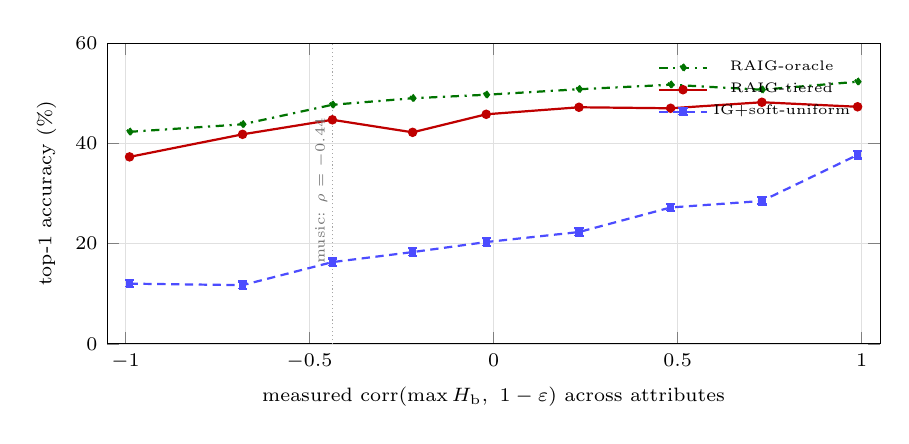
\begin{tikzpicture}
\begin{axis}[
  width=0.94\columnwidth, height=5.4cm,
  xlabel={measured $\mathrm{corr}(\max\Hb,\ 1-\varepsilon)$ across attributes},
  ylabel={top-1 accuracy (\%)},
  xmin=-1.05, xmax=1.05, ymin=0, ymax=60,
  xtick={-1,-0.5,0,0.5,1},
  tick label style={font=\scriptsize}, label style={font=\scriptsize},
  legend style={font=\tiny, at={(0.98,0.98)}, anchor=north east, draw=none,
                fill=none, row sep=-1pt},
  grid=major, grid style={black!12, very thin},
  mark size=1.3pt,
]
\addplot[green!45!black, thick, dashdotted, mark=diamond*] coordinates
  {(-0.989,42.3) (-0.682,43.8) (-0.438,47.7) (-0.220,49.0) (-0.020,49.7)
   (0.232,50.8) (0.481,51.7) (0.729,50.7) (0.989,52.3)};
\addlegendentry{RAIG-oracle}
\addplot[red!75!black, thick, mark=*] coordinates
  {(-0.989,37.3) (-0.682,41.8) (-0.438,44.7) (-0.220,42.2) (-0.020,45.8)
   (0.232,47.2) (0.481,47.0) (0.729,48.2) (0.989,47.3)};
\addlegendentry{RAIG-tiered}
\addplot[blue!70, thick, densely dashed, mark=square*] coordinates
  {(-0.989,12.0) (-0.682,11.7) (-0.438,16.3) (-0.220,18.3) (-0.020,20.3)
   (0.232,22.3) (0.481,27.2) (0.729,28.5) (0.989,37.7)};
\addlegendentry{IG+soft-uniform}
\draw[black!35, thin, densely dotted] (axis cs:-0.438,0) -- (axis cs:-0.438,60);
\node[font=\tiny, anchor=south west, black!55, rotate=90]
  at (axis cs:-0.425,14) {music: $\rho=-0.44$};
\end{axis}
\end{tikzpicture}
\caption{The advantage as a continuous function of the informativeness/
reliability correlation, on a synthetic catalogue family with everything else
held fixed. Classical information gain degrades monotonically as the
correlation turns adversarial, from $37.7\%$ at $\rho=+0.99$ to $12.0\%$ at
$\rho=-0.99$. Reliability-aware selection is close to flat over the same range
($47.3\%$ to $37.3\%$). The correlation therefore measures how badly classical
selection is \emph{harmed}, not whether the correction is \emph{available};
the dotted line marks the correlation measured on the music catalogue.}
\label{fig:rho}
\end{figure}
%----------------------------------------------------------------------

The sweep contains no break-even point. RAIG-tiered leads at every setting,
from $+9.67\pp$ at $\rho = +0.99$---where the informative attributes are also
the reliable ones and there is, on the correlation account, nothing to
correct---to $+30.17\pp$ at $\rho = -0.68$. That is the same lesson the
cross-domain results gave, now on a controlled axis: what the correlation
governs is the \emph{denominator}, how far classical information gain falls,
not whether reliability-aware selection has anything to offer. And the reason
the correction is always available here is the one the previous paragraph
identifies---in this family twelve of the twenty attributes fall in the
reliable tiers and place $76\%$ to $94\%$ of items in a singleton class, so
steering towards them is affordable at every $\rho$.

The practical reading combines the two experiments. A catalogue with an
adversarial correlation \emph{and} an answerable reliable subset is the best
case, and it is where the music catalogue sits. A catalogue with an answerable
reliable subset but no correlation still benefits, and that is dermatology. A
catalogue whose reliable subset cannot identify anything does not benefit
whatever its correlation, and that is mushroom.

\subsection{Abstention}
\label{sec:results-erasure}

Section~\ref{sec:erasure} derives the acquisition function for a user who may
decline to answer, \eqref{eq:erasure}, and attaches a prediction to it: if
abstention correlates with subjectivity in the same direction as error, the two
penalties compound and the bias should be \emph{larger} than the pure-BSC
analysis suggests. Predictions of that kind belong in an experiment rather than
in a future-work list, so we implement the channel and test it. Each attribute
additionally returns an erasure with probability $\delta_f$, tied to its tier
on the reasoning that a user who cannot judge an attribute reliably is also the
one most likely to decline it; an erased turn is consumed but produces no
belief update. Three selectors are compared: classical information gain, blind
to both; RAIG, which models error but not abstention; and RAIG+erasure, which
models both.

\begin{table}[t]
\caption{The abstention channel. Mild is $\delta = (0.02, 0.10, 0.20)$ by tier,
strong is $(0.05, 0.20, 0.40)$; the error channel is heterogeneous
$\lambda = 1.0$ throughout, $n = 450$ paired trials. ``Answered'' is the
fraction of consumed turns that returned an answer rather than an erasure, and
is a consequence of which questions the selector chose.}
\label{tab:erasure}
\centering
\footnotesize
\begin{tabular}{@{}llrrr@{}}
\toprule
\textbf{Abstention} & \textbf{Method} & \textbf{acc.\ (\%)} &
\textbf{answered} & \textbf{subj.\ \%} \\
\midrule
none   & IG+soft-uniform & 2.44 & 1.000 & 53.4 \\
       & RAIG-tiered     & 7.78 & 1.000 & 2.8 \\
       & RAIG+erasure    & 7.78 & 1.000 & 2.8 \\
\midrule
mild   & IG+soft-uniform & 1.56 & 0.849 & 54.3 \\
       & RAIG-tiered     & 5.33 & 0.930 & 1.8 \\
       & RAIG+erasure    & 4.00 & 0.932 & 1.2 \\
\midrule
strong & IG+soft-uniform & 1.11 & 0.692 & 55.6 \\
       & RAIG-tiered     & 4.00 & 0.854 & 1.4 \\
       & RAIG+erasure    & 3.56 & 0.862 & 0.5 \\
\bottomrule
\end{tabular}
\end{table}

Table~\ref{tab:erasure} reports the outcome. There are two results, and the
first is a refutation of our own prediction.

\emph{The absolute advantage shrinks rather than grows.} RAIG-tiered leads
IG+soft-uniform by $+5.33\pp$ with no abstention, $+3.78\pp$ under mild
abstention and $+2.89\pp$ under strong abstention. Measured on the paper's
headline scale, the penalties do not compound; they compress, because
abstention pushes every method towards the floor and there is progressively
less accuracy to win. The prediction of Section~\ref{sec:erasure} is wrong as
stated, and we let it stand in the theory section rather than quietly deleting
it, because the version that survives is worth having: on a \emph{relative}
scale the compounding is real and monotone, with RAIG's accuracy $3.18\times$
IG's without abstention, $3.43\times$ under mild and $3.60\times$ under strong.
The right conclusion is that abstention makes classical selection relatively
worse and absolutely no more distinguishable, which is a weaker claim than the
one we made in advance.

\emph{Modelling abstention explicitly buys nothing here.} RAIG+erasure is
indistinguishable from RAIG-tiered with no abstention (identical, as it must be
when $\delta \equiv 0$) and slightly \emph{worse} under both mild
($-1.33\pp$, $p = 0.24$) and strong ($-0.44\pp$, $p = 0.80$) abstention. Neither
difference is significant, so the finding is an absence rather than a reversal,
but the point estimate is in the wrong direction and the mechanism is
instructive. Because $\delta_f$ is tied to the tier in the same order as
$\varepsilon_f$, the error-based discount has already steered the selector away
from the high-abstention questions: RAIG-tiered gets $93.0\%$ of its turns
answered under mild abstention against classical selection's $84.9\%$, without
modelling abstention at all. The extra $(1-\delta)$ factor then applies a
second discount to attributes that are already being avoided, driving the
subjective share of questions to $0.5\%$ at strong abstention and narrowing the
question pool towards the reliable-subset ceiling of
Section~\ref{sec:results-synthetic}---the same over-correction that produces
the clean-condition collapse.

The practical implication is that a deployed system facing abstention should
model it in the \emph{belief update}, where an erasure must not be treated as
evidence, and can safely leave the selector to the error term alone---provided
abstention and error are ordered the same way across attributes. Where they
are not, \eqref{eq:erasure} is the correct criterion and this experiment says
nothing against it.

\subsection{Correlated Answer Errors}
\label{sec:results-correlated}

The channel of Section~\ref{sec:method} draws every answer independently at
rate $\varepsilon$. A real listener who misjudges ``is it energetic?'' is
likely to misjudge it the same way when asked again, so independence is the
modelling assumption most likely to be flattering to us, and it should be
attacked directly rather than listed as a limitation.

We attack it with a deliberately harsh alternative. The first time a
\emph{subjective} attribute is answered wrongly in a session, that attribute is
marked corrupted for the remainder of the session and every later question
about it is forced wrong; objective and semi-objective attributes keep
independent draws, since simple slips rather than conceptual confusion are the
plausible failure there. This turns a rate-$\varepsilon$ channel into a
per-session absorbing one on exactly the attributes classical selection
prefers. Both variants run inside the same loop and consume the same random
stream in the same order, so the independent and correlated columns are paired
trial for trial and any difference between them is the correlation and nothing
else.

The result, in Table~\ref{tab:correlated}, strengthens rather than weakens the
paper's conclusion.

\begin{table}[t]
\caption{Independent against correlated answer errors, heterogeneous
$\lambda = 1.0$, $n = 900$, paired trial for trial across all four cells.
Correlating errors on subjective attributes costs classical selection
$0.78\pp$ and costs reliability-aware selection exactly nothing.}
\label{tab:correlated}
\centering
\footnotesize
\begin{tabular}{@{}lrrr@{}}
\toprule
\textbf{Method} & \textbf{independent} & \textbf{correlated} &
\textbf{difference} \\
\midrule
IG+soft-uniform & 2.78 & 2.00 & $-0.78\pp$ ($p = 0.016$) \\
RAIG-tiered     & 7.78 & 7.78 & $+0.00\pp$ ($p = 1.00$) \\
\midrule
$\Delta$ (RAIG $-$ IG) & $+5.00\pp$ & $+5.78\pp$ & \\
McNemar $p$ & $3.6\times10^{-7}$ & $3.1\times10^{-9}$ & \\
\bottomrule
\end{tabular}
\end{table}

Correlating the errors costs IG+soft-uniform $0.78\pp$---seven trials that it
won under independent errors and loses under correlated ones, and not a single
trial in the other direction---while RAIG-tiered's outcome is
\emph{bitwise identical} across the two variants: zero discordant pairs out of
$900$. The paired advantage therefore grows from $+5.00\pp$ to $+5.78\pp$, and
its $p$-value improves by two orders of magnitude.

The asymmetry is not luck, and it follows from Table~\ref{tab:asked}. The
absorbing mechanism can only fire on subjective attributes. Classical selection
spends $53.9\%$ of its budget there and is exposed to it on most turns;
RAIG-tiered spends $2.9\%$ and is almost never exposed, and in these $900$
sessions it was never exposed twice to the same subjective attribute, which is
what a repeat requires. A selector that avoids the attributes on which users
are unreliable is, as a side effect, also robust to their errors being
persistent rather than fresh---which is a property worth having, since
persistence is the more realistic model and the harder one to estimate.

We do not claim this exhausts the question. Errors could correlate
\emph{across} attributes rather than within one---a listener with an unusual
notion of ``energetic'' probably also has an unusual notion of
``danceable''---and that structure would penalise any method that clusters its
questions within a tier, including ours. Testing it would require a
user-level latent-trait model that we do not have data to fit.

\subsection{An Online Alternative to the Tiers, and Its Catalogue-Size Dependence}
\label{sec:results-streaming}

Section~\ref{sec:results-em} removes the three assumed tier values by learning
a crossover vector \emph{offline}, from six hundred already-completed
sessions, before the vector is ever used. A natural sharper version of the
same idea is to skip the offline pass entirely: re-estimate the per-attribute
crossover \emph{online}, from the trials the deployed system is already
running, with no tier annotation assumed even as a cold-start value. We built
and tested exactly this variant, \textbf{RAIG-streaming}, and report both what
happened and why, because the failure is as informative as a success would
have been.

\emph{The mechanism.} Every attribute starts at a single neutral crossover,
$\hat\varepsilon = 0.10$, no tiers involved. Between batches of paired
trials---not inside the per-turn loop itself, which would couple the estimate
to a single session's own noise---the same attribute-pooled
expected-disagreement statistic Section~\ref{sec:results-em} computes offline
is folded into a running per-attribute total, and the estimate used by the
NEXT batch is the resulting mean, shrunk toward the neutral prior with a
pseudo-count of sixty so that an attribute with little evidence cannot swing
on a handful of noisy readings. A fraction of turns, $20\%$, is forced to a
uniformly random available question regardless of the current estimate,
mirroring the forced-exploration fix Section~\ref{sec:results-em}'s offline
estimator already needed for the identical reason.

\emph{On the full catalogue, it loses, to a diagnosed mechanism rather than to
noise.} At the primary condition and $T=70$ (Table~\ref{tab:streaming}),
RAIG-streaming reaches $18.56\%$ against RAIG-tiered's $38.56\%$---a
$20.00\pp$ deficit, exact McNemar $p = 5.0\times10^{-27}$---and even trails
plain classical information gain's $27.11\%$ by $8.56\pp$
($p = 4.4\times10^{-6}$). The cause is a feedback loop the fixed tiers cannot
experience because they never move. \texttt{genre} alone compiles to $113$ of
the catalogue's $193$ questions and is genuinely the most reliable attribute
in it; the moment the running estimate correctly notices this, the selector
asks it more, which supplies more evidence for exactly that attribute and
none for the other nineteen, whose own estimates stay noisy and drift toward
the unreliable end of the clip range from thin, badly-timed samples. Measured
directly over these $900$ sessions, \texttt{genre} takes $58.6\%$ of every
question RAIG-streaming asks, against $36.0\%$ for the curator's fixed tiers
and $24.6\%$ for classical information gain at the same operating
point---a share no fixed annotation ever produces, because a fixed annotation
cannot compound the way a live one can. An earlier, unregularised attempt
(no shrinkage, $10\%$ exploration) put \texttt{genre}'s share at $78.7\%$ and
reached only $5.9\%$ accuracy; the shrinkage-and-exploration fix reported here
roughly triples that, but does not close the gap to the tiers at this scale.

\begin{table}[t]
\caption{Static tiers against the online alternative, primary condition,
$T=70$, $n=900$. $\Delta$ and $p$ are against RAIG-tiered, exact McNemar,
Holm-corrected within this family.}
\label{tab:streaming}
\centering
\footnotesize
\begin{tabular}{@{}lrrr@{}}
\toprule
\textbf{Method} & \textbf{top-1 (\%)} & \textbf{$\Delta$ (pp)} & \textbf{$p$ (Holm)} \\
\midrule
IG+soft-uniform            & 27.11 & $-11.44$ & $5.1\times10^{-9}$  \\
RAIG-streaming             & 18.56 & $-20.00$ & $5.0\times10^{-27}$ \\
RAIG-streaming+stop@0.5    & 19.78 & $-18.78$ & $5.2\times10^{-24}$ \\
RAIG-streaming+stop@0.7    & 18.00 & $-20.56$ & $1.2\times10^{-28}$ \\
RAIG-streaming+stop@0.9    & 17.78 & $-20.78$ & $1.2\times10^{-28}$ \\
\textbf{RAIG-tiered}       & \textbf{38.56} & --- & --- \\
\bottomrule
\end{tabular}
\end{table}

\emph{Raising the cap alone, on the tiers, is the clean win in this
experiment.} RAIG-tiered itself improves from $26.56\%$ at the budget of
Table~\ref{tab:primary} to $38.56\%$ simply by raising $T$ from $40$ to $70$
with nothing else changed---an operating-point change, not a methodological
one, and the only unambiguous gain reported in this subsection.

\emph{Early stopping at $T=70$ behaves exactly as
Section~\ref{sec:results-behaviour} predicts it will at $T=20$: it mostly
does not fire.} A confidence threshold of $0.90$ crosses in $1.1\%$ of
RAIG-streaming sessions by turn seventy; $0.70$ in $2.0\%$; $0.50$ in $3.6\%$.
None of the three changes accuracy by a significant amount relative to
running the streaming estimator to completion (Table~\ref{tab:streaming}, all
$p_{\text{Holm}} = 1.00$). Forty additional questions past the entropy floor
still mostly does not buy the confidence a stopping rule needs to act on; it
buys accuracy at a fixed budget instead, which is the mechanism
Table~\ref{tab:streaming} already reports.

\emph{The deficit is not fixed: it is catalogue-size dependent.}
Section~\ref{sec:results-size} already reports that the RAIG-over-IG
advantage survives at every catalogue size tested. We repeated the
online-versus-static comparison specifically, on an independently drawn
$5{,}000$-item subset (identifiability ceiling $99.5\%$, floor $12.28$ bits)
with the budget extended to $T=200$ (Table~\ref{tab:streamsize}). The pattern
reverses: by $T=80$ the two are statistically indistinguishable ($71.00\%$
against $71.44\%$, $p = 0.85$), and the gap stays indistinguishable from zero
through $T=200$ ($73.89\%$ against $72.67\%$, $p = 0.52$)---RAIG-streaming's
point estimate is even fractionally higher at the longest budget tested, but
not significantly so. We do not claim the online estimator wins at small
scale; we report that the deficit it shows at full scale is not a fixed
property of the method, and that a smaller identification task gives the
same online estimator enough of its own budget to reach parity with an
annotation it was never given.

\begin{table}[t]
\caption{The online estimator against static tiers on a $5{,}000$-item
subset, one independent draw, $n=900$, primary condition. $p$ is the exact
McNemar test between RAIG-streaming and RAIG-tiered at that column.}
\label{tab:streamsize}
\centering
\footnotesize
\begin{tabular}{@{}lrrrrr@{}}
\toprule
\textbf{Method} & \textbf{$T{=}40$} & \textbf{$T{=}60$} & \textbf{$T{=}80$} &
\textbf{$T{=}100$} & \textbf{$T{=}200$} \\
\midrule
IG+soft-uniform  & 41.33 & 56.67 & 58.44 & 58.44 & 58.00 \\
RAIG-tiered      & 61.33 & 69.56 & 71.44 & 72.89 & 72.67 \\
RAIG-streaming   & 47.89 & 64.89 & 71.00 & 72.11 & 73.89 \\
\midrule
$p$ (streaming vs.\ tiered) & --- & --- & $0.85$ & $0.71$ & $0.52$ \\
\bottomrule
\end{tabular}
\end{table}

\emph{Reading the two results together.} What the online estimator lacks
relative to the offline one of Section~\ref{sec:results-em} is repetition:
the offline estimator replays the same fixed logged sequence eight times,
each pass recomputing belief under a better crossover guess; the online one
sees every trial once, under whichever guess happened to be current when
that trial ran. On a catalogue small enough, or a budget long enough, that a
single pass supplies adequate coverage of every attribute, this costs little.
On the full catalogue at $T=70$ it costs a great deal, because
\texttt{genre}'s dominance of the question pool gives the feedback loop room
to run before the other nineteen attributes accumulate enough evidence to
compete. We report this as a diagnosed limitation with a concrete next
step---an online estimator that replays its own most recent batch a small,
fixed number of times before committing to the next one, borrowing the
offline estimator's repetition without its six-hundred-session
latency---rather than as a closed question.

%=============================================================================
\section{Discussion}
\label{sec:discussion}
%=============================================================================

\subsection{What This Paper Establishes}

Four things, the first three in decreasing order of confidence and the fourth
the one that answers the objection this work is most exposed to.

That \emph{classical information gain systematically solicits the questions
users answer worst, in catalogues of a particular shape}, is established by
direct measurement of selector behaviour and does not depend on any assumed
$\varepsilon$. On the music catalogue, a classical selector asks questions
whose annotated crossover averages $0.225$ against a catalogue average of
$0.098$, filling $53.9\%$ of a twenty-question budget with the tier a listener
judges least reliably, while a uniformly random selector faces $0.097$, which
is the catalogue average. Whatever one believes about the numeric values of
$\varepsilon$, the ordering of the annotation is what drives that contrast, and
the contrast is large.

That \emph{the effect is manufactured by discretisation rather than inherited
from the domain} is established by three independent lines that agree:
Proposition~\ref{prop:discretisation}, which shows quantile binning fixes
apparent informativeness at $\Hb(1/k)$ irrespective of semantics; the
measurement that binned attributes carry mean maximum information gain $0.861$
against $0.618$ for natively categorical ones; and the observation that
refining the binning to four equal-population bins \emph{strengthens} the
measured bias, from $\rho = -0.44$ to $\rho = -0.61$. The absence of the effect
in two catalogues with no continuous attributes to bin is the prediction this
account makes, and it holds.

That \emph{correcting the acquisition function helps, and does so from an
annotation cheap enough to be deployable}, is established at $n=900$ paired
trials with exact tests and multiplicity control, and---more importantly---is
shown to survive the assumption it rests on: over $60$ worlds drawn from priors
on the tier values, the fixed deployed system wins in $60$ of $60$, with a
minimum advantage of $+1.33\pp$. Three coarse tiers recover roughly $72\%$ of
what perfect per-attribute knowledge would deliver, and a two-tier annotation
recovers $78\%$ of the three-tier gain (Section~\ref{sec:results-ablation}).

That \emph{the three assumed constants are not load-bearing} is answered three
ways, in increasing strength: the conclusion survives
a distribution over those constants; it survives a majority of attributes being
placed in the wrong tier; and the constants are not required at all. EM over
$600$ logged sessions of the already-deployed incumbent---no annotation, no
labels, and the target item latent throughout---recovers a per-attribute
crossover vector that matches the curator's annotation to a dead heat, $38$
discordant pairs in each direction out of $900$
(Section~\ref{sec:results-em}).

Two of the model's structural assumptions were attacked directly, and the
outcomes point in opposite directions. Relaxing independence across turns
\emph{strengthens} the result: making subjective errors persist for the rest of
a session costs classical selection $0.78\pp$ and costs reliability-aware
selection exactly nothing, because a selector that avoids unreliable attributes
is not exposed to their errors being persistent
(Section~\ref{sec:results-correlated}). Adding abstention, by contrast, refutes
a prediction we made in advance: we expected the penalties to compound and the
absolute advantage to grow, and it shrinks
(Section~\ref{sec:results-erasure}). Only the relative advantage compounds. We
report the failed prediction because a paper that only tests the predictions it
expects to confirm is not testing anything.

\subsection{What It Does Not Establish}

We claim no algorithmic novelty. The acquisition function is the mutual
information between the target and the observed answer under a binary symmetric
channel; it is in Cover and Thomas~\cite[Ch.~7]{cover2006}, and a reader who
finds \eqref{eq:raig} unsurprising is reading it correctly. The contribution is
that the observation model in some deployed attribute catalogues is
heterogeneous in a specific and adversarial way, that the heterogeneity is
partly an artefact of preprocessing, that a learned policy trained without a
noise model inherits the blind spot, and that the correction needs far less
knowledge about users than one would expect. Those are empirical claims, and
they are what the experiments are for.

Nor have we measured $\varepsilon$ on people, and it is worth being precise
about what the log-based estimator of Section~\ref{sec:results-em} does and
does not settle. It establishes identifiability and sufficiency: a
per-attribute crossover vector can be recovered from six hundred sessions of
ordinary use without annotation, labels or ground truth, and recovering it is
enough to match a hand-annotated one exactly. It does not establish that real
users behave this way, because the logs it consumes were generated by a
simulator whose users err at rates drawn from the annotation---so what EM
recovers is, at bottom, the structure we put in. The same caveat applies to
the ensemble over tier priors (Section~\ref{sec:results-ensemble}), the
corruption sweep (Section~\ref{sec:results-corruption}) and the repeated-item
measurement (Section~\ref{sec:reliability-empirical}). Together they establish
that the conclusion is not an artefact of three particular numbers. None of
them tells a practitioner what $\varepsilon$ is in their domain, and only the
study of Appendix~\ref{app:protocol} would.

Finally, the two negative results on catalogue-derived specifications should
not be softened, because together they say something the positive results do
not. RAIG-empirical, which infers reliability from the rate at which repeated
items disagree with each other, is beaten by the three-tier annotation by
$6.33\pp$ and is no better than classical information gain. RAIG-psycho, which
computes the crossover of each binned attribute from the position of its own
cut points, fails at every setting of its two parameters
(Section~\ref{sec:results-psycho}). Both measure a property of the
\emph{catalogue}, and both are defeated by the same thing: a listener cannot
name the key of a song, not because the boundary between keys is fuzzy or
because the catalogue disagrees with itself about it, but because they never
learned to name keys. Answerability is a fact about people. What succeeds---the
curator's tiers, and the vector learned from logs---succeeds because each is,
in the end, an observation of people rather than of data.

\subsection{A Deployment Test}

The cross-domain results yield a procedure a practitioner can run before
committing to anything, and it is the most transferable output of this work.

\begin{enumerate}
\item \emph{Is there anything to correct?} Compute per-attribute maximum
one-versus-rest entropy and compare it across a coarse answerability
annotation. A Kruskal--Wallis test on three tiers is the right instrument; a
Spearman correlation on three tied levels is not. If informativeness
concentrates on the hard-to-answer tier, classical selection is being actively
misled.
\item \emph{Is the correction affordable in information?} Compute the
identifiability ceiling of the reliable attribute subset by counting distinct
attribute vectors. This costs one database query. If the ceiling is high
(dermatology, $70.8\%$), reliability-aware selection will help substantially
even when step~1 finds no bias. If it is near zero (mushroom, $0.3\%$), the
unreliable attributes are load-bearing and no selection rule can route around
them.
\item \emph{Is the channel actually noisy?} Reliability weighting is a
correction for a noisy channel and is harmful when the channel is clean: in our
clean condition RAIG-tiered loses to classical selection by more than
fifty points at $T=20$, because it breaks ties towards attributes that cannot
by themselves separate the catalogue. Switch it off, not down, when answers are
reliable.
\item \emph{Annotate coarsely and ship, then let the system re-estimate.} Two
tiers recover $78\%$ of what three tiers deliver, and three tiers recover about
$72\%$ of what per-attribute truth would deliver. Once the system is running,
that residual is addressable without a measurement campaign: EM over its own
logs recovers a per-attribute vector that matches the annotation
(Section~\ref{sec:results-em}). The order of operations is therefore curator
first, logs second, user study only if the first two disagree.
\end{enumerate}

Steps~1 and~2 are computable from the catalogue alone. Step~3 requires knowing
roughly how noisy users are, which is the one thing that genuinely needs
observation---and Section~\ref{sec:results-lambda} locates the threshold.

\subsection{Threats to Validity}

\emph{Simulated users.} Every session in this paper is played by a simulator
drawing from a binary symmetric channel. This is the central threat and we do
not minimise it. Its severity is bounded in three ways: the deployed system
never sees the true $\varepsilon$; the conclusion is reported across a
distribution of true $\varepsilon$ rather than at a point; and two structural
assumptions of the channel---that every turn is an independent draw, and that a
question is always answered---are attacked directly in
Sections~\ref{sec:results-correlated} and~\ref{sec:results-erasure}. Three
things remain unaddressed. Whether real answer errors are well described by
\emph{any} per-attribute rate is the deepest of them, and only the study of
Appendix~\ref{app:protocol} can settle it. The channel is assumed
\emph{symmetric}, whereas real users may well have a bias---readier to say
``yes'' than ``no'' when unsure---which an asymmetric binary channel would
capture and which our formulation does not. And errors are correlated within an
attribute in Section~\ref{sec:results-correlated} but never \emph{across}
attributes, though a listener with an unusual notion of ``energetic'' plausibly
has an unusual notion of ``danceable'' too; that structure would penalise any
method that concentrates its questions within a tier, ours included.

\emph{One primary catalogue.} The headline comparison is on music. We add two
further catalogues and a synthetic family precisely because one catalogue
cannot support a general claim, and the resulting scope condition is stated as
a condition rather than as a universal.

\emph{Greedy selection.} We select greedily throughout. Greedy optimality under
noise is established for a single common crossover probability~\cite{jedynak2012}
and, as Remark~\ref{rem:greedy} notes, does not obviously extend to
heterogeneous per-attribute capacities. Holding the policy class fixed at the
one deployed systems use is what isolates the acquisition function; it is not a
claim that greedy is optimal here.

\emph{Static reliability.} $\hat\varepsilon$ is fixed for the session. A real
system could estimate a user's per-attribute reliability online from answer
consistency, which would make the specification problem largely disappear---and
would introduce an exploration/exploitation trade-off this paper does not
address.

\emph{Simulator--method coupling.} The simulator and the method share the
functional form of the noise model. This is standard in the noisy-search
literature but it is a real limitation: the ensemble experiment breaks the
parameter coupling but not the functional-form coupling, and the abstention
experiment is the only place where the true channel has a component the
baseline selector cannot represent.

\subsection{Future Work}

The obvious next step is the user study, and it is specified rather than
gestured at. Beyond it, three directions follow from what the experiments
showed rather than from what would be conventional to list.

\emph{Per-user} reliability estimation is the most valuable, and is the natural
extension of what Section~\ref{sec:results-em} already does. That estimator
pools every session into one crossover vector, which is the right object when
the population is homogeneous and the wrong one when it is not: a musician and
a casual listener do not share a crossover for ``what key is it in''. Estimating
$\hat\varepsilon_f$ per user, from within-session answer consistency and a
population prior, is a hierarchical version of the same EM and would attack the
variation this paper's model cannot express. It also introduces an
exploration/exploitation trade-off---questions asked to learn about the user
rather than about the item---that Section~\ref{sec:results-em} shows is not
free, and Section~\ref{sec:results-streaming} shows can be worse than not
free: we tried the simpler, non-hierarchical version of this idea---one
crossover vector, updated \emph{online} from the deployment's own trials
instead of offline from a fixed log---and it loses badly on the full
catalogue to a feedback loop the offline estimator's repeated replay does not
allow (\texttt{genre} monopolises $58.6\%$ of every question asked once the
running estimate correctly favours it, starving the other nineteen
attributes of the evidence needed to estimate them), though the deficit
disappears on a smaller catalogue with a longer budget. A per-user version
would face the identical loop at the scale of a single session rather than
the whole deployment, which is a reason for pessimism about a naive
implementation and a concrete requirement---replay, or an explicit
optimism bonus for under-sampled attributes, not exploration alone---for a
serious one.

Non-myopic selection under heterogeneous capacities is the most interesting
theoretically. Corollary~\ref{cor:budget} makes the difficulty concrete: with
per-attribute capacities, a horizon-optimal policy may wish to reserve a
high-capacity attribute for a later turn when the belief can exploit it, and a
greedy rule cannot express that preference.

Finally, the discretisation result suggests attacking the problem one stage
earlier. If quantile binning is what manufactures the bias, then a
reliability-aware \emph{discretiser}---one that chooses bin boundaries to
maximise mutual information through the channel rather than to equalise
populations---would prevent it rather than compensate for it. Nothing in this
paper requires the binning to be given.

%=============================================================================
\section{Conclusion}
\label{sec:conclusion}
%=============================================================================

Expected information gain is the default acquisition function for interactive
identification, and it was derived for an oracle that answers exactly. When the
oracle is a person, the criterion has a blind spot with a specific shape: it
scores a question by how evenly it divides the belief, and vagueness is what
makes a split even. In a catalogue that mixes quantile-binned perceptual
descriptors with skewed categorical metadata, the criterion therefore seeks out
the questions users answer worst---not as a failure of tuning but as a
consequence of what it optimises, sharpened by a preprocessing step that fixes
apparent informativeness at a value determined by the bin count rather than by
the attribute.

The correction is a single line, and it is textbook: score the question by the
mutual information between the target and the observed answer through a
per-attribute binary symmetric channel. What we have tried to establish is not
that this quantity is new but that it is needed, and that the knowledge it
requires is cheap enough to be had. Two coarse tiers recover most of the
benefit; the annotation may be wrong for a majority of attributes before it
stops paying; across sixty worlds drawn from priors on the tier values a system
shipping the fixed point estimates wins in sixty; and a two-line audit of the
catalogue predicts in advance whether any of this will help. The three numbers
need not even be assumed: EM over six hundred logged sessions of the
already-deployed incumbent, with the target item latent and nothing annotated,
recovers a crossover vector that matches the curator's exactly.

We have also been explicit about the boundaries. Reliability weighting is a
correction for a noisy channel, and on a clean one it is not merely useless but
harmful. It requires a reliability model, and inverting that model inverts the
result. The two routes that would have supplied one from the catalogue
alone---repeated-item instability, and a psychophysical model of the bin
boundaries---both fail, and fail for the same reason: they measure the data,
and answerability is a property of the people. The route that does work without
a curator is to watch those people, which is what the log-based estimator does
and why it succeeds where the catalogue-derived ones do not. And the parameter
has still not been measured on real people, only on simulated ones. That is the
piece of work this paper specifies and does not do, and it is the piece that
would close the argument.

%=============================================================================
\appendices
%=============================================================================

\section{A Protocol for Measuring $\varepsilon_f$ from Users}
\label{app:protocol}

The most exposed assumption of this paper is the tier annotation
$(0.03, 0.15, 0.30)$, and four experiments reduce the exposure without removing
it. Section~\ref{sec:reliability-empirical} measures an adjacent quantity from
the catalogue; Section~\ref{sec:results-ensemble} shows the conclusion survives
a distribution over the values; Section~\ref{sec:results-corruption} shows how
wrong the tier assignment can be before the correction stops paying; and
Section~\ref{sec:results-em} dispenses with the values entirely, recovering
them from interaction logs.

None of that is the same as measuring $\varepsilon_f$ on people, and the last
of the four is the one whose limits are easiest to overstate. Its logs come
from a simulator whose users err at rates drawn from the annotation, so it
establishes that the parameter is \emph{identifiable} from logs of that size
and that recovering it \emph{suffices}, not that human error rates have this
shape. Only observation of people can establish that. We did not run a human
study, and rather than list that as a limitation we specify the study, so that
the gap is a piece of work someone can do rather than a hole in the argument.

\subsection*{Design}

The estimand is not ``how often is a user wrong'', which is unidentifiable
without ground truth about what the user is thinking. It is the crossover
probability of the channel between the item a user has in mind and the answer
they give: $\varepsilon_f = \Pr[\,\tilde{a}_f \neq a_f(c) \mid c\,]$, where
$a_f(c)$ is the catalogue's value and $\tilde{a}_f$ the user's report. This is
identifiable if the item is known to the experimenter and unknown to be under
test by the participant.

\emph{Task.} A participant is shown a track---title, artist, and a
thirty-second audio excerpt---and asked the same one-versus-rest binary
questions the deployed system would ask, in randomised order. Because the
catalogue value $a_f(c)$ is known, each answer is directly scoreable, and
$\hat\varepsilon_f$ is the per-attribute error rate with a Wilson
interval~\cite{wilson1927}.

\emph{Recall versus perception.} A user of the deployed system answers from
memory, not from an excerpt. The excerpt condition therefore measures a lower
bound on $\varepsilon_f$. We would run both arms: a \emph{perception} arm with
the excerpt available, and a \emph{recall} arm in which participants nominate
tracks they claim to know well and answer without hearing them. The contrast
between the arms is itself the interesting quantity for objective attributes,
where the excerpt makes the answer nearly free but recall does not.

\emph{Sample size.} To separate the annotated tiers we need to distinguish
$0.03$ from $0.15$ and $0.15$ from $0.30$. At $\varepsilon = 0.15$, a Wilson
interval of half-width $0.05$ requires roughly $200$ answers per attribute.
With $20$ attributes and $30$ questions per participant, that is $130$--$140$
participants, or fewer if each answers about several tracks. A pilot at $n=25$
would not resolve individual attributes but would resolve the \emph{tier
contrast}, which is what the method actually consumes: pooling within tiers
gives roughly $1{,}300$ answers per tier at $n=25$, ample to reject tier
equality.

\emph{Analysis.} The per-attribute rate is a proportion with a Wilson interval;
the tier contrast is a mixed-effects logistic regression with a random
intercept per participant and per track, since answers from the same person and
about the same track are not independent. The pre-registered test is the tier
main effect. The secondary analysis regresses $\hat\varepsilon_f$ on (i) the
annotated tier, (ii) the measured catalogue discordance $d_f$ of
\eqref{eq:discordance}, and (iii) the bin count of the attribute, which is the
direct test of the psychophysical mechanism of
Section~\ref{sec:psychophysical}.

\subsection*{What the Study Would and Would Not Settle}

It would settle whether the three-tier ordering is real and roughly how far
apart the tiers are, which is the only property of the annotation that the
method uses: by Proposition~\ref{prop:uniform} only the heterogeneity does any
work, by Section~\ref{sec:results-em} an estimate that is correctly ordered but
badly calibrated performs as well as the truth, and by
Section~\ref{sec:results-corruption} the tier assignment may be wrong for most
attributes before the correction stops paying. The study needs to establish an
ordering, not three decimal places, and it is powered accordingly.

It would not settle the point values for a different catalogue, a different
population, or a different interface, and it should not be read as doing so.
The transportable claim in this paper is conditional and has two parts, which
Section~\ref{sec:results-synthetic} separates. Where answerability is
heterogeneous \emph{and} negatively aligned with apparent informativeness,
classical selection is actively misled and the correction pays most. Where it
is heterogeneous but unaligned, classical selection is merely blind and the
correction still pays, provided the answerable attributes carry enough
information to finish the job. Where they do not, no selection rule can route
around them. Three coarse tiers capture most of the available gain in the first
two cases, and nothing helps in the third.

\section{Reproduction}
\label{app:repro}

Every number in this paper is produced by a script in the released repository
and stored as JSON, and the tables are checked against those files
mechanically rather than transcribed by hand. The determinism requirements of
Section~\ref{sec:system}---single-threaded BLAS, externally supplied random
streams---make the runs bitwise reproducible on a given machine and make each
method's results invariant to which other methods are run alongside it.

Two caveats are worth recording. First, results generated before the
single-thread pin was introduced do not reproduce bitwise; they agree within
sampling error, and where such a run is quoted we say so. Second, the budget
sweep, the $\varepsilon$-ensemble and the cross-domain comparisons are
independent runs at their own sample sizes, so their overlapping cells agree
within sampling error rather than exactly. We report the overlaps rather than
suppressing them.


\bibliographystyle{IEEEtran}
\bibliography{refs}

\end{document}
